
\documentclass[Tese.tex]{subfiles}

\begin{document}
	
\chapter{Modelo viscoelástico-viscoplástico} \label{ch:vep}

\begin{figure}[!b]
	\centering
	\caption{Modelo reológico visco-elasto-plástico}
	\label{fig:modelo-reologico}
	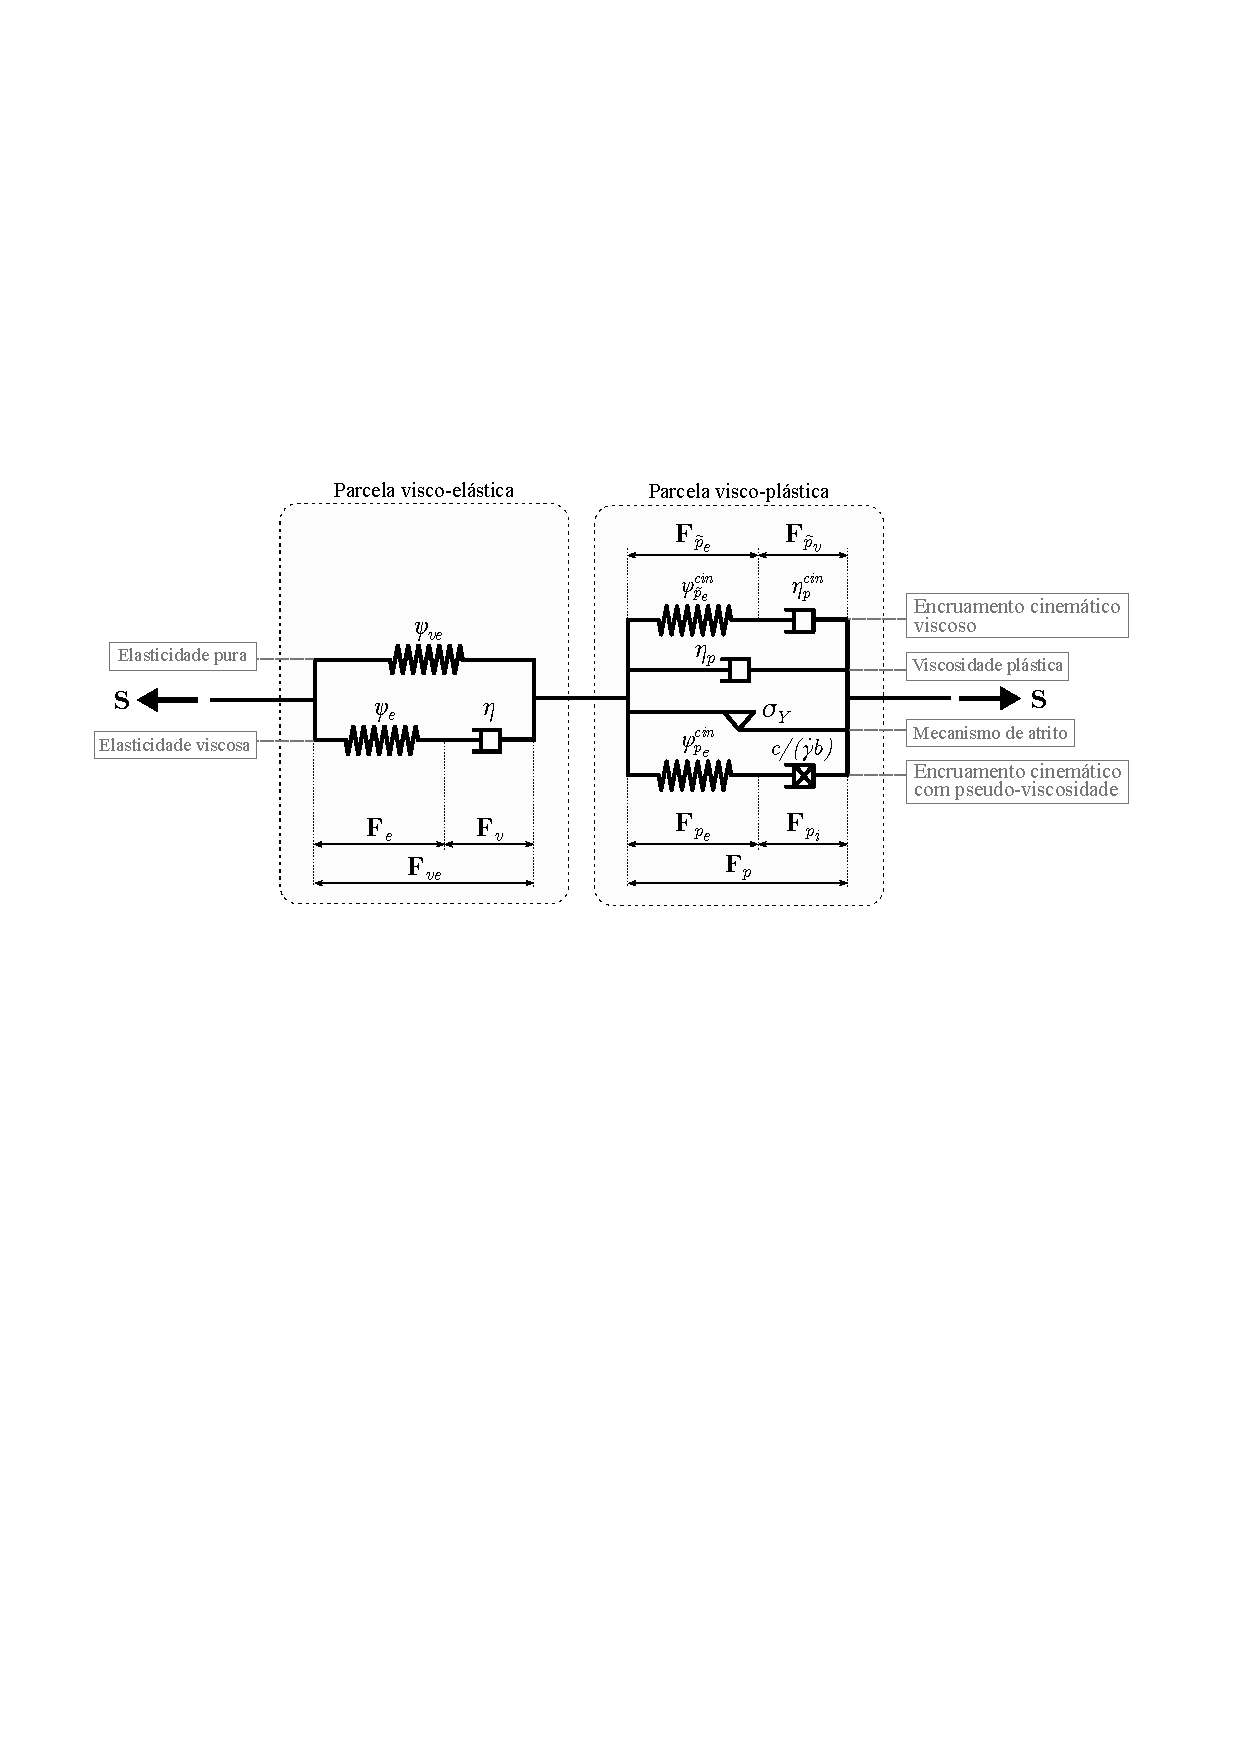
\includegraphics[scale=0.9]{Figuras/modelo-reologico.pdf}
	\caption*{\textbf{Fonte:} Adaptado de \citeonline{Pericles2019}}
\end{figure}

O modelo viscoelástico-viscoplástico apresentado neste trabalho é baseado no de \citeonline{Pericles2019}, sendo adicionada uma parcela de encruamento cinemático viscoso a fim de contemplar a dependência temporal da rigidez plástica. 

Assim, constrói-se o modelo reológico que serve como base para os desenvolvimentos desta seção, apresentado na \autoref{fig:modelo-reologico}. Esse modelo consiste na associação em série de uma parcela viscoelástica, representada pelo modelo de Zener \textcolor{red}{colocar referência e identificar na figura (Zener) abaixo de Parcela visco-elástica}, e uma viscoplástica. A plasticidade é simbolizada por um mecanismo de atrito, e a viscoplasticidade é considerada pela associação em paralelo desse mecanismo de atrito com um pistão de viscosidade $\viscplast$. Além disso, baseado na proposta de \citeonline{Lion1997}, é possível decompor as deformações plásticas em parcelas ``plásticas-elásticas'' e ``plásticas-inelásticas'', que representam, na micro-escala, as deformações induzidas por discordâncias e as deformações irreversíveis devidas a escorregamentos nos cristais, respectivamente. Com essa ideia, é possível incorporar no modelo a lei de encruamento cinemático de Armstrong-Frederick \textcolor{red}{incluir citação}, considerando que as parcelas plásticas-elásticas são representadas por uma mola com rigidez ``$\armstrongstiff$'' e as parcelas plásticas-inelásticas por um pistão com viscosidade ``$\armstrongstiff/(\plastmult\armstrongvisc)$''. Observa-se, no entanto, que esse pistão não evolui com o tempo, mas sim com o nível das deformação plástica, tratando-se portanto de uma pseudo-viscosidade. Dessa forma, considera-se associado em paralelo um modelo adicional de encruamento cinemático viscoso, onde a parcela de deformação plástica-inelástica é representada por um pistão de viscosidade $\visccin$ variável no tempo. 

A adição do encruamento cinemático viscoso permite que o modelo apresentado seja aplicado com precisão ao material politetrafluoretileno (PTFE), cujos resultados experimentais mostram uma notável dependência das taxas de deformação sobre a rigidez plástica. Isso é demonstrado na \autoref{sec:validacao}, após a descrição completa do modelo constitutivo.

\section{Cinemática}\label{sec:cinematica-vep}
Por ser aplicado a problemas com grandes deformações, utiliza-se neste modelo a decomposição multiplicativa como apresentada na \autoref{subsec:dec-mult-termo-elastico} aplicada ao caso termo-elástico. Nesse contexto, o gradiente da função mudança de configuração é expresso como:

\textcolor{red}{Sugiro colocar deformação no singular sempre que estiver se referindo a um único caso ou ao modelo reológico. As componentes do tensor são componentes da medida de deformação e não das deformações... O mesmo se aplica a tensão. Assim, fica no plural só quando for genérico (ex.: grandes deformações, tensões elevadas... Não vou modificar mais isso daqui pra frente, fica por sua conta se você preferir assim.)}


\begin{equation}
\F = \Fve\Fp. \label{eq:dec-mult-1}
\end{equation}
onde $\Fve$ corresponde à parcela viscoelástica de deformação, e $\Fp$ denota a parcela plástica, ou viscoplástica. Além disso, baseado no modelo reológico adotado, as deformações viscoelásticas podem ser decompostas em parcelas elásticas ($\Fe$) e viscosas ($\Fv$), isto é,
\begin{equation}
\Fve = \Fe\Fv, \label{eq:dec-mult-2}
\end{equation}
e as deformações plásticas podem ser decompostas em parcelas plásticas-elásticas e plásticas-inelásticas, conforme comentado anteriormente, de duas formas:
\begin{equation}
\Fp = \Fpe\Fpi = \Fpve\Fpvi, \label{eq:dec-mult-3}
\end{equation}
onde a primeira decomposição é utilizada para representar o encruamento cinemático pseudo-viscoso, e a segunda o encruamento cinemático viscoso. Conforme discutido na \autoref{subsec:dec-mult-termo-elastico}, cada decomposição multiplicativa está associada a uma configuração intermediária do sólido. Na \autoref{fig:kinematics-vep} essas configurações intermediárias são apresentadas de forma esquemática com os seus respectivos mapeamentos.

\begin{figure}[!htb]
	\centering
	\caption{Configurações intermediárias para a decomposição multiplicativa aplicada ao modelo constitutivo viscoelástico-viscoplástico}
	\label{fig:kinematics-vep}
	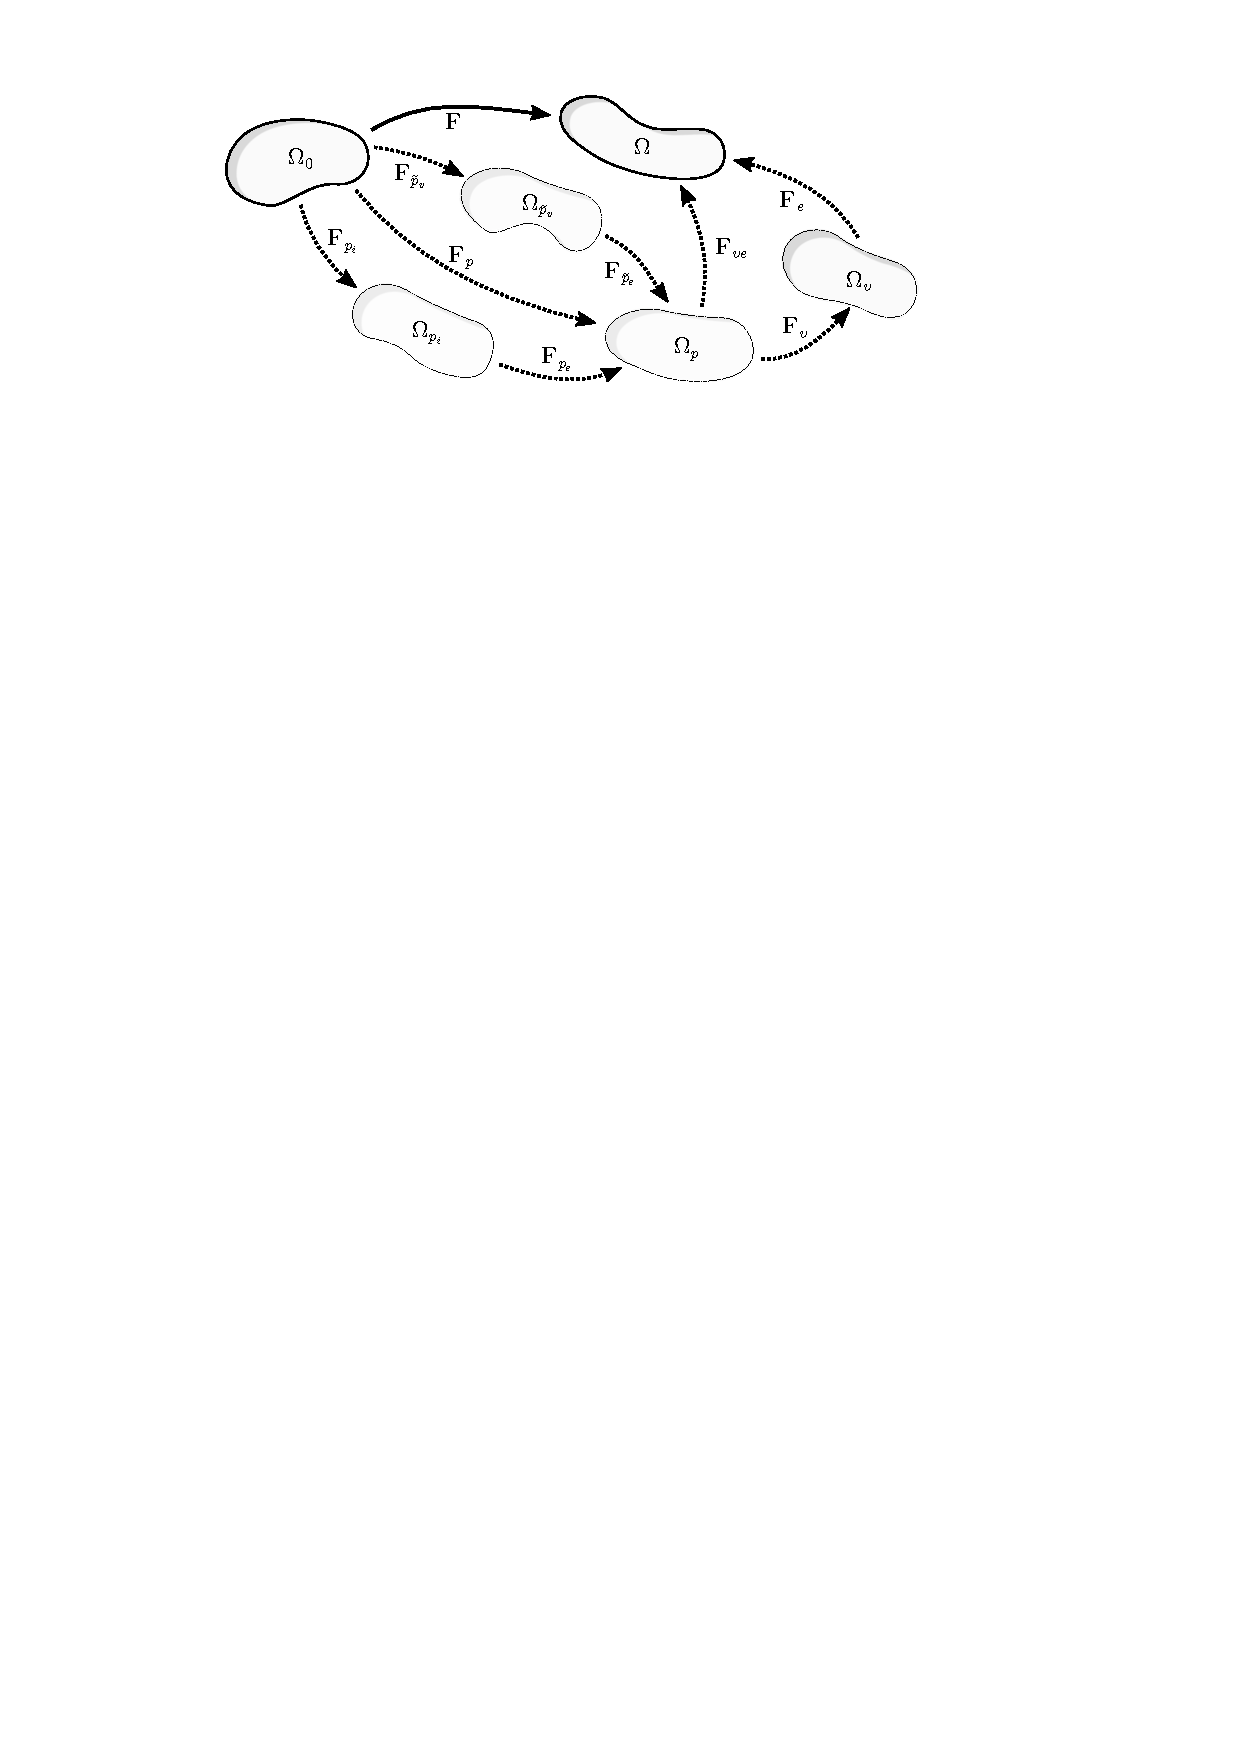
\includegraphics[scale=1.04]{Figuras/kinematics-vep.pdf}
	\caption*{\textbf{Fonte:} Adaptado de \citeonline{Pericles2019}}
\end{figure}

Para cada parcela apresentada do gradiente da função mudança de configuração, denotada de forma genérica por $\F_{(\cdot)}$, pode-se definir tensores associados ao alongamento à direita de Cauchy-Green, $\C_{(\cdot)}$, à deformação de Green-Lagrange, $\E_{(\cdot)}$, à velocidade da mudança de configuração, $\L_{(\cdot)}$, e à taxa de deformação de engenharia, $\D_{(\cdot)}$, por expressões análogas às Eqs. \eqref{eq:alongamentocauchy}, \eqref{eq:E}, \eqref{eq:gradiente-velocidade} e \eqref{eq:taxa-deformacao}, respectivamente. 

%Assim, pela decomposição da \cref{eq:dec-mult-1}, podemos obter as seguintes relações:
%\begin{align}
%&\C = (\Fve\Fp)^T(\Fve\Fp) = \Fp^T\Cve\Fp,\\
%&\L = \dotF\F^{-1} = (\dotFve\Fp + \Fve\dotFp)(\Fve\Fp)^{-1} = \Lve + \Fve\Lp\Fve^{-1} \text{,\quad e}\\
%&\D = \Sim(\L) = \Dve + \Sim(\Fve\Lp\Fve^{-1}). \label{eq:D-relacao}
%\end{align}
%Aplicando as \cref{eq:dec-mult-1,eq:taxa-green-2} na \cref{eq:D-relacao}, e desenvolvendo algebricamente, é possível escrever a taxa da deformação de Green-Lagrange viscoelástica como
%\begin{equation}
%\dotEve = \Fp^{-T}\dotE\Fp^{-1} - \Sim(\Cve\Lp). \label{eq:dotEve}
%\end{equation}
%Realizando procedimentos análogos para a decomposições das \cref{eq:dec-mult-2,eq:dec-mult-3}, podemos também escrever
%\begin{align}
%&\dotEe = \Fv^{-T}\dotEve\Fv^{-1} - \Sim(\Ce\Lv),\label{eq:dotEe} \\
%&\dotEpe = \Fpi^{-T}\dotEp\Fpi^{-1} - \Sim(\Cpe\Lpi) , \text{\; e} \label{eq:dotEpe} \\
%&\dotEpve = \Fpvi^{-T}\dotEp\Fpvi^{-1} - \Sim(\Cpve\Lpvi). \label{eq:dotEpve}
%\end{align}

\section{Energia, tensão e dissipação}

Com base na \autoref{fig:modelo-reologico}, é possível expressar a energia livre de Helmholtz do modelo constitutivo por meio das parcelas de energia armazenadas nas quatro molas apresentadas. Na parcela viscoelástica, essas parcelas são denotadas por $\helmholtzve$ e $\helmholtze$, sendo a primeira associada às deformações viscoelásticas totais, e a segunda apenas às deformações elásticas. Para a parcela viscoplástica, temos as molas $\helmholtzkinv$ e $\helmholtzkin$, responsáveis pelo encruamento cinemático viscoso e pseudo-viscoso, respectivamente. Adicionalmente, a fim de representar o encruamento isotrópico, pode-se considerar uma energia armazenada $\helmholtzisop$, dependente apenas de um parâmetro de encruamento $\encruamento$. Assim, a energia livre de Helmholtz pode ser escrita como:
\begin{equation}\label{eq:helmholtz-vep}
\helmholtz = \helmholtzve(\Eve) + \helmholtze(\Ee) + \helmholtzkin(\Epe) + \helmholtzkinv(\Epve) + \helmholtzisop(\encruamento).
\end{equation}
É importante ser dito que as parcelas de energia apresentadas são originalmente definidas nas suas respectivas configurações intermediárias. No entanto, como será visto posteriormente, as deformações inelásticas são isocóricas, isto é, preservam o volume da configuração inicial. Portanto, a quantidade de energia por unidade de volume nas configurações intermediárias é igual à quantidade de energia por unidade de volume na configuração inicial, permitindo que as parcelas $\helmholtzve$, $\helmholtze$, $\helmholtzkin$ e $\helmholtzkinv$ possam ser definidas sem que haja qualquer preocupação relacionada à conversão de volumes, ao contrário do caso termo-elástico (\autoref{subsec:dec-mult-termo-elastico}).

Propõe-se neste trabalho um modelo termodinamicamente consistente, isto é, cujas equações respeitem as leis da termodinâmica. Em particular, deve ser atendida a inequação de Clausius-Duhem, escrita para o caso isotérmico na \cref{eq:clausius-duhem-iso}. Para isso, é necessário calcular taxa da energia livre de Helmholtz. Com base na \cref{eq:helmholtz-vep}, escreve-se:
\begin{equation}\label{eq:dotHelmholtz-0}
\dothelmholtz = \dfrac{\partial \helmholtzve}{\partial \Eve}:\dotEve + \dfrac{\partial \helmholtze}{\partial \Ee}:\dotEe + \dfrac{\partial \helmholtzkin}{\partial \Epe}:\dotEpe + \dfrac{\partial \helmholtzkinv}{\partial \Epve}:\dotEpve + \dfrac{\partial \helmholtzisop}{\partial \encruamento}\dotencruamento.
\end{equation}

Utilizando-se as relações cinemáticas obtidas pela decomposição multiplicativa, acrescidas de manipulações algébricas na \cref{eq:dotHelmholtz-0}, discutidas com mais detalhes em \citeonline{Pericles2019}, a inequação de Clausius-Duhem pode ser expressa por:
\begin{equation}
\begin{aligned}
\dissipation = & \left(\S-\Fp^{-1}\dfrac{\partial \helmholtzve}{\partial \Eve}\Fp^{-T}-\Fp^{-1}\Fv^{-1}\dfrac{\partial \helmholtze}{\partial \Ee}\Fv^{-T}\Fp^{-T}\right):\dotE + \left(\Ce\dfrac{\partial \helmholtze}{\partial \Ee} \right):\Lv \\&+ \left(\Cve\dfrac{\partial \helmholtzve}{\partial \Eve} + \Fv^T\Ce\dfrac{\partial \helmholtze}{\partial \Ee}\Fv^{-T} - \Fpe\dfrac{\partial \helmholtzkin}{\partial \Epe}\Fpe^{T} - \Fpve\dfrac{\partial \helmholtzkinv}{\partial \Epve}\Fpve^{T}\right):\Lp  \\&+ \left( \Cpe\dfrac{\partial \helmholtzkin}{\partial \Epe} \right):\Lpi  + \left(\Cpve\dfrac{\partial \helmholtzkinv}{\partial \Epve}\right):\Lpvi - \dfrac{\partial \helmholtzisop}{\partial \encruamento}\dotencruamento \geq 0. \label[ineq]{eq:dint-0}
\end{aligned}
\end{equation}
Conforme postulado por \citeonline{Coleman1963}, a inequação acima deve ser válida para qualquer processo termodinâmico, isto é, qualquer valor de $\dotE$. Dessa forma, para garantir a não-negatividade do primeiro termo da \cref{eq:dint-0}, esse é igualado a zero. Isso implica que a tensão de Piola-Kirchhoff de segunda espécie deve ser dada por:
\begin{equation}
\S = \Fp^{-1}\dfrac{\partial \helmholtzve}{\partial \Eve}\Fp^{-T} + \Fp^{-1}\Fv^{-1}\dfrac{\partial \helmholtze}{\partial \Ee}\Fv^{-T}\Fp^{-T}, \label{eq:S-vep}
\end{equation}
e a \cref{eq:dint-0} pode ser reescrita como:
\begin{equation}
\dissipation = \mandele:\Lv + \relativeStress:\Lp + \mandelpe:\Lpi + \mandelpve:\Lpvi + \yieldStress\dotencruamento \geq 0, \label[ineq]{ineq:dint}
\end{equation}
onde 
\begin{equation}
\yieldStress = -\dfrac{\partial\helmholtzisop}{\partial\encruamento},
\end{equation}
$\relativeStress$ é denominado tensão relativa, definido como:
\begin{equation}
\relativeStress = \mandelve + \Fv^T\mandele\Fv^{-T} - \Fpe\dfrac{\partial \helmholtzkin}{\partial \Epe}\Fpe^{T} - \Fpve\dfrac{\partial \helmholtzkinv}{\partial \Epve}\Fpve^{T}, \label{eq:relativeStress}
\end{equation}
e os demais tensores são definidos por \begin{equation}
\mandele = \Ce\dfrac{\partial \helmholtze}{\partial \Ee},\quad \mandelve = \Cve\dfrac{\partial \helmholtzve}{\partial \Eve},\quad \mandelpe = \Cpe\dfrac{\partial \helmholtzkin}{\partial \Epe} \quad\text{e}\quad \mandelpve = \Cpve\dfrac{\partial \helmholtzkinv}{\partial \Epve} \label{eq:mandel}
\end{equation}
sendo denominados tensores de Mandel, definidos nas suas respectivas configurações intermediárias. Para modelos isotrópicos, é possível verificar que os tensores de Mandel são simétricos \cite{SVENDSEN1998473}. A partir da \cref{ineq:dint}, diz-se que $\relativeStress$ é a medida de tensão termodinamicamente conjugada à $\Lp$, sendo, portanto, utilizada para definir o critério de escoamento do modelo constitutivo.

\section{Critério de escoamento e leis de evolução}\label{sec:leis-evolucao}

Utiliza-se neste trabalho o critério de escoamento de von Mises, definido no presente contexto pela seguinte função:
\begin{equation}\label{eq:yield}
\yield = \|\relativeStressD\| - \sqrt{\dfrac{2}{3}}\left(\yieldStresscte - \yieldStress\right),
\end{equation}
onde $\yieldStresscte$ é a tensão de escoamento, e o sobrescrito $(\cdot)\desviador$ denota a parcela desviadora de um tensor. No caso de plasticidade independente de taxa \textcolor{red}{(Explicar melhor: você quer dizer no caso das parcelas viscosas associadas com o mecanismo de atrito serem nulas? A taxa a que você se refere é a taxa de deformação plástica? A parcela viscoelástica continua presente (dependente da taxa de deformação)?)}, tem-se a condição $\yield \leq 0$. Já no caso da viscoplasticidade, em particular no modelo de Perzyna \textcolor{red}{(Você não definiu o modelo de Perzyna ainda no seu trabalho. Precisa definir ele em algum lugar antes dessa sentença.)), esse critério é substituído por uma lei viscosa, como será visto adiante.

Para que a \cref{ineq:dint} seja atendida, expressões adequadas devem ser escolhidas para $\Lv$, $\Lp$, $\Lpi$, $\Lpvi$ e $\dotencruamento$, chamadas leis de evolução. Ainda, utilizando a relação $\L_{(\cdot)} = \dotF_{(\cdot)}\F_{(\cdot)}^{-1}$, é possível escrever essas expressões utilizando as taxas de cada componente do gradiente da função mudança de configuração. Uma forma intuitiva de obter as leis de evolução é pelo princípio da máxima dissipação da energia, discutido com detalhes em \citeonline{Pericles2019}. Para a lei de evolução viscosa, pode-se tomar
\begin{equation}
	\Lv = \dfrac{1}{\visc}\mandeleD \qquad\text{ou}\qquad \dotFv = \dfrac{1}{\visc}\mandeleD\Fv. \label{eq:Lv-evol}
\end{equation}
onde $\visc$ é o parâmetro de viscosidade. Para a lei de evolução plástica, pode-se tomar
\begin{equation}
\Lp = \plastmult\Np  \qquad\text{ou}\qquad \dotFp = \plastmult\Np\Fp \label{eq:Lp-evol}
\end{equation}
onde $\Np = {\relativeStressD}/{\|\relativeStressD\|}$ é o tensor que controla a direção da evolução plástica e $\plastmult$ é o multiplicador plástico. Seguindo o modelo viscoplástico de \citeonline{PERZYNA1966243}, o multiplicador plástico é dado por $\plastmult = {\langle\overstress\rangle}/{\viscplast}$, onde $\viscplast$ é o parâmetro de viscosidade plástica, $\langle\cdot\rangle$ denota o colchete de Macaulay, isto é, $\langle\overstress\rangle = (\overstress + |\overstress|)/2$, e $\overstress$ é denominada função das tensões excedentes (\emph{overstress}), definida em função de $\yield$ e escolhida de forma que seja contínua e convexa para $\yield\geq 0$, e nula quando $\yield = 0$. Neste trabalho, adota-se
\begin{equation}
\overstress = e^{\overstresscte\yield}-1,
\end{equation}
onde $\overstresscte$ é um parâmetro de calibração do material. 

Para as parcelas de encruamento cinemático pseudo-viscoso e viscoso, as leis de evolução são tomadas, respectivamente, como
\begin{align}
\Lpi = \plastmult\dfrac{\armstrongvisc}{\armstrongstiff}\mandelpeD \qquad&\text{ou}\qquad \dotFpi = \plastmult\dfrac{\armstrongvisc}{\armstrongstiff}\mandelpeD\Fpi \label{eq:Lpi-evol}\\[0.1cm]
\Lpvi = \dfrac{1}{\visccin}\mandelpveD \qquad&\text{ou}\qquad \dotFpvi = \dfrac{1}{\visccin}\mandelpveD\Fpvi. \label{eq:Lpvi-evol}
\end{align}
A \cref{eq:Lpi-evol} é uma generalização da lei de encruamento cinemático de Armstrong-Frederick para o caso de grandes deformações, sendo $\armstrongstiff$ a constante de rigidez plástica, e $\armstrongvisc$ um parâmetro adimensional. Observa-se que a \cref{eq:Lpvi-evol} não depende do multiplicador plástico $\plastmult$, logo, mesmo tratando-se de uma variável plástica, o tensor $\Lpvi$ pode ser não-nulo ainda que o material não esteja em regime plástico. 

Por fim, a lei de evolução do encruamento isotrópico é dada por:
\begin{align}
	\dotencruamento = \sqrt{\dfrac{2}{3}}\plastmult. \label{eq:evol-iso}
\end{align}

Para que o modelo apresentado seja termodinamicamente consistente, deve-se ainda garantir que este respeite a segunda lei da termodinâmica. Para isso, aplicam-se as \cref{eq:Lv-evol,eq:Lp-evol,eq:Lpi-evol,eq:Lpvi-evol,eq:evol-iso} na \cref{ineq:dint}, de onde, utilizando a propriedade tensorial $\mathbf{A}:\mathbf{A}\desviador = \|\mathbf{A}\desviador\|^2$, resulta
\begin{equation}
\dissipation = \plastmult\|\relativeStressD\| + \dfrac{1}{\visc}\|\mandeleD\|^2 + \plastmult\dfrac{\armstrongvisc}{\armstrongstiff}\|\mandelpeD\|^2 + \dfrac{1}{\visccin}\|\mandelpveD\|^2 + \sqrt{\dfrac{2}{3}}\plastmult\yieldStress. \label{eq:dint-verif}
\end{equation}

A partir do critério de escoamento, \cref{eq:yield}, tem-se que $\plastmult\|\relativeStressD\| + \sqrt{\frac{2}{3}}\plastmult\yieldStress = \plastmult\yield + \sqrt{\frac{2}{3}}\plastmult\yieldStresscte$, que é maior ou igual a zero dada a definição de $\plastmult$. Como todos os demais termos da \cref{eq:dint-verif} também são maiores ou iguais a zero, a condição $\dissipation \geq 0$ é satisfeita. 

Utilizando um procedimento análogo ao apresentado em \citeonline{Pericles2019}, é possível demonstrar que as leis de evolução adotadas garantem a propriedade da conservação do volume inelástico, ou seja, $\Jp$, $\Jv$, $\Jpi$ e $\Jpvi$ são unitários, onde $\J_{(\cdot)}=\det\F_{(\cdot)}$ denota o determinante Jacobiano de cada parcela da deformação.

\section{Solução numérica}\label{sec:solucao-numerica}

A integração temporal das leis de evolução é realizada neste trabalho pelo método implícito de Euler, também chamado neste contexto de algoritmo de retorno radial. Aplicando esse método às \cref{eq:Lv-evol,eq:Lp-evol,eq:Lpi-evol,eq:Lpvi-evol,eq:evol-iso} escreve-se as formas discretas no tempo:
\begin{align}
& \Rv = \Fv-\Fv\indprev - \dfrac{\Delta t}{\visc}\mandeleD\Fv = \mathbf{0}, \label{eq:evol-Fv-disc}\\[0.1cm]
& \Rp = \Fp - \Fp\indprev - \dplastmult\Np\Fp = \mathbf{0}, \label{eq:evol-Fp-disc}\\[0.1cm]
& \Rpi = \Fpi - \Fpi\indprev - \dplastmult\dfrac{\armstrongvisc}{\armstrongstiff}\mandelpeD\Fpi = \mathbf{0}, \label{eq:evol-Fpi-disc}  \\[0.1cm]
& \Rpvi = \Fpvi - \Fpvi\indprev - \dfrac{\Delta t}{\visccin}\mandelpveD\Fpvi = \mathbf{0}, \text{\; e}  \label{eq:evol-Fvi-disc} \\[0.1cm]
& \Renc = \encruamento - \encruamento\indprev - \dplastmult\sqrt{\dfrac{2}{3}} = 0, \label{eq:evol-encruamento-disc}
\end{align}
onde $\Rv$, $\Rp$, $\Rpi$, $\Rpvi$ e $\Renc$ são os resíduos do sistema não-linear, os termos com índice sobrescrito $(\cdot)\indprev$ são tomados no instante anterior do passo de tempo, enquanto os demais termos são tomados no instante atual, sendo $\Delta t$ o intervalo do passo de tempo, e $\dplastmult = \plastmult\Delta t$.

Nos passos de tempo onde ocorre plastificação, adiciona-se ainda a condição de consistência. Para materiais com plasticidade independente de taxa, tem-se:
\begin{equation}\label{eq:comp1}
\Rplastmult = \yield = 0.
\end{equation}
Já para materiais viscoplásticos com modelo de Perzyna, essa condição é substituída por:
\begin{equation}\label{eq:comp2}
\Rplastmult = \dplastmult - \Delta t\dfrac{\langle\overstress\rangle}{\viscplast} = 0.
\end{equation}


 
O algoritmo desenvolvido baseia-se em etapas de previsão e correção, apresentado em forma de fluxograma na \autoref{fig:fluxograma-vep}. Deve ser mencionado que o método implícito de Euler provoca erros numéricos na propriedade da conservação do volume inelástico \cite{DETTMER200487,Vladimirov}, e, portanto, requer um passo de tempo suficientemente pequeno grande para evitar discrepâncias, como pode ser visto nas análises realizadas em \citeonline{Tsakmakis2003} e \citeonline{Pericles2019}.

\begin{figure}[!htb]
	\centering
	\caption{Fluxograma do algoritmo previsão-correção para marcha no tempo}
	\label{fig:fluxograma-vep}
	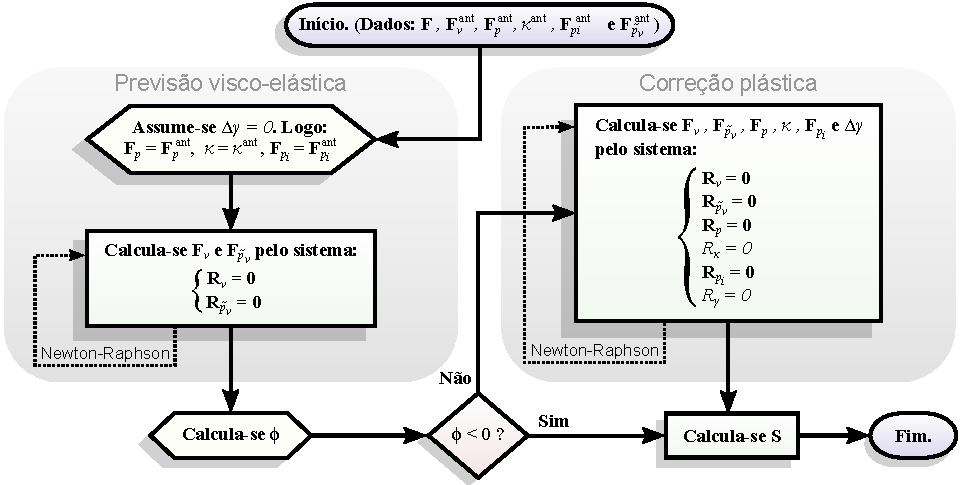
\includegraphics[scale=0.98]{Figuras/fluxograma-vep.pdf}
	%\caption*{\textbf{Fonte:} Elaborado pelo autor}
\end{figure}

\section{Operador tangente consistente}\label{sec:operador-vep}

Para garantir convergência ótima da solução numérica com o modelo constitutivo não linear, o operador tangente consistente, representado pelo tensor de quarta ordem $\CC$, é definido de tal forma que:
\begin{equation}\label{eq:CC-vep-0}
\Delta\S = \CC:\Delta\E
\end{equation}
onde $\Delta\S$ e $\Delta\E$ são, respectivamente, as variações no passo de tempo da tensão de Piola-Kirchhoff de segunda espécie e da deformação de Green-Lagrange.

Utilizando as relações cinemáticas descritas na \cref{sec:cinematica-vep}, é possível escrever $\S$ apenas em função de $\E$, $\Fv$ e $\Fp$. Assim, vale a seguinte aproximação de primeira ordem:
\begin{equation}\label{eq:dS}
\Delta\S \approx \dfrac{\partial\S}{\partial\E}:\Delta\E + \dfrac{\partial\S}{\partial\Fv}:\Delta\Fv + \dfrac{\partial\S}{\partial\Fp}:\Delta\Fp.
\end{equation}
Para que a \cref{eq:dS} possa ser associada à forma da \cref{eq:CC-vep-0}, deve-se expressar $\Delta\Fv$ e $\Delta\Fp$ em termos de $\Delta\E$. Esse processo não é trivial, exigindo determinadas manipulações algébricas sobre as leis de evolução e de consistência. 

No contexto numérico, a condição de consistência pode ser expressa como
\begin{equation}
\dplastmult\Delta\Rplastmult=0.
\end{equation}
Essa condição implica que, caso o material esteja em regime plástico, e portanto $\dplastmult>0$, $\Delta\Rplastmult$ deve ser nulo. No caso viscoplástico, $\Rplastmult$ é dado pela \cref{eq:comp2}. Dessa forma, o valor de $\Delta\Rplastmult$ pode ser aproximado por:
\begin{equation}
\dfrac{\partial\Rplastmult}{\partial\E}:\Delta\E + \dfrac{\partial\Rplastmult}{\partial\Fv}:\Delta\Fv + \dfrac{\partial\Rplastmult}{\partial\Fp}:\Delta\Fp + \dfrac{\partial\Rplastmult}{\partial\kappa}\Delta\kappa + \dfrac{\partial\Rplastmult}{\partial\Fpi}:\Delta\Fpi + \dfrac{\partial\Rplastmult}{\partial\Fpvi}:\Delta\Fpvi + \dfrac{\partial\Rplastmult}{\partial\plastmultsymbol}\dplastmult \approx 0.\label{eq:deltaRplast}
\end{equation}
Além disso, como $\Rv$ e $\Rpvi$ devem ser nulos para todo passo de tempo, também deve ser válido que $\Delta\Rv = \mathbf{0}$ e $\Delta\Rpvi = \mathbf{0}$. Tendo em vista que $\Rv$ pode ser escrito apenas em termos de $\E$, $\Fv$ e $\Fp$, e que $\Rpvi$ pode ser escrito apenas em termos de $\Fp$ e $\Fpvi$, as seguintes aproximações podem ser aplicadas:
\begin{align}
&\dfrac{\partial\Rv}{\partial\E}:\Delta\E + \dfrac{\partial\Rv}{\partial\Fv}:\Delta\Fv + \dfrac{\partial\Rv}{\partial\Fp}:\Delta\Fp \approx \mathbf{0},\text{\quad e}  \\[0.1cm]
&\dfrac{\partial\Rpvi}{\partial\Fp}:\Delta\Fp + \dfrac{\partial\Rv}{\partial\Fpvi}:\Delta\Fpvi \approx \mathbf{0},
\end{align}
de onde resulta:
\begin{align}
&\Delta\Fv \approx -\left(\dfrac{\partial\Rv}{\partial\Fv}\right)^{-1}:\left(\dfrac{\partial\Rv}{\partial\E}:\Delta\E + \dfrac{\partial\Rv}{\partial\Fp}:\Delta\Fp\right),\text{\quad e} \label{eq:deltaFv}\\[0.1cm]
&\Delta\Fpvi \approx -\left(\dfrac{\partial\Rpvi}{\partial\Fpvi}\right)^{-1}:\left(\dfrac{\partial\Rpvi}{\partial\Fp}:\Delta\Fp\right). \label{eq:deltaFpvi}
\end{align} 

Aplicando-se as \cref{eq:deltaFv,eq:deltaFpvi} na \cref{eq:deltaRplast}, e substituindo as variações $\Delta\Fp$, $\Delta\kappa$ e $\Delta\Fpi$ pelas leis de evolução discretizadas \eqref{eq:evol-Fp-disc}, \eqref{eq:evol-encruamento-disc} e \eqref{eq:evol-Fpi-disc}, chega-se a:
\begin{equation}
\DE:\Delta\E + \Dgamma\dplastmult \approx 0 \label{eq:De-Dgamma-aprox}
\end{equation}
onde
\begin{align}
&\DE = \dfrac{\partial\Rplastmult}{\partial\E} - \dfrac{\partial\Rplastmult}{\partial\Fv}:\left(\dfrac{\partial\Rv}{\partial\Fv}\right)^{-1}:\dfrac{\partial\Rv}{\partial\E},\text{\quad e}\\[0.1cm]
&\begin{aligned}
 \Dgamma = & \left[\dfrac{\partial\Rplastmult}{\partial\Fp} -  \dfrac{\partial\Rplastmult}{\partial\Fv}:\left(\dfrac{\partial\Rv}{\partial\Fv}\right)^{-1}:\dfrac{\partial\Rv}{\partial\Fp} - \dfrac{\partial\Rplastmult}{\partial\Fpvi}:\left(\dfrac{\partial\Rpvi}{\partial\Fpvi}\right)^{-1}:\dfrac{\partial\Rpvi}{\partial\Fp}\right]:\left(\Np\Fp\right) \\ &+ \dfrac{\partial\Rplastmult}{\partial\encruamento}\sqrt{\dfrac{2}{3}} + \dfrac{\armstrongvisc}{\armstrongstiff}\dfrac{\partial\Rplastmult}{\partial\Fpi}:\left(\mandelpeD\Fpi\right) +  \dfrac{\partial\Rplastmult}{\partial\plastmultsymbol}.
\end{aligned}
\end{align}

Da \cref{eq:De-Dgamma-aprox}, segue-se que
\begin{equation}
\dplastmult \approx \Dplastmult:\Delta\E,
\end{equation}
onde $\Dplastmult = -\DE/\Dgamma$ é um tensor que pode ser interpretado, para passos de tempo suficientemente pequenos, como a derivada de $\plastmultsymbol$ com relação a $\E$. Assim, pela lei de evolução discretizada de $\Fp$, tem-se:
\begin{equation}
\Delta\Fp = \dplastmult\Np\Fp \approx (\Dplastmult:\Delta\E)\Np\Fp = \left[\left(\Np\Fp\right)\otimes\Dplastmult\right]:\Delta\E. \label{eq:dFp-dE-0}
\end{equation}
Aplicando a \cref{eq:dFp-dE-0} na \cref{eq:deltaFv}, resulta:
\begin{equation}
\Delta\Fv \approx -\left(\dfrac{\partial\Rv}{\partial\Fv}\right)^{-1}:\left[\dfrac{\partial\Rv}{\partial\E} + \dfrac{\partial\Rv}{\partial\Fp}:\left(\Np\Fp\right)\otimes\Dplastmult\right]:\Delta\E, \label{eq:dFv-dE-0}
\end{equation}
e, finalmente, aplicando as \cref{eq:dFp-dE-0,eq:dFv-dE-0} na \cref{eq:dS}, e associando-a com a \cref{eq:CC-vep-0}, define-se o operador tangente consistente do modelo viscoelástico-viscoplástico pela seguinte expressão:
\begin{equation}
\CC = \dfrac{\partial\S}{\partial\E} - \dfrac{\partial\S}{\partial\Fv}:\left(\dfrac{\partial\Rv}{\partial\Fv}\right)^{-1}:\left[\dfrac{\partial\Rv}{\partial\E} + \dfrac{\partial\Rv}{\partial\Fp}:\left(\Np\Fp\right)\otimes\Dplastmult\right] + \dfrac{\partial\S}{\partial\Fp}:\left(\Np\Fp\right)\otimes\Dplastmult. \label{eq:CC-vep}
\end{equation}

Por fim, deve-se considerar os passos de tempo nos quais não houve correção plástica, isto é, $\dplastmult=0$. Nesses casos, temos $\Dplastmult=\mathbf{0}$, logo a \cref{eq:CC-vep} pode ser simplificada para
\begin{equation}
\CC = \dfrac{\partial\S}{\partial\E} - \dfrac{\partial\S}{\partial\Fv}:\left(\dfrac{\partial\Rv}{\partial\Fv}\right)^{-1}:\dfrac{\partial\Rv}{\partial\E}.
\end{equation}

\aquiii
\section{Definição da energia livre de Helmholtz}\label{sec:helmholtz-vep}

Para finalizar a descrição do modelo constitutivo, resta definir as expressões para cada parcela da energia livre de Helmholtz. Em geral, as parcelas $\helmholtzve$, $\helmholtze$, $\helmholtzkin$ e $\helmholtzkinv$ são dadas por leis hiperelásticas definidas em termos das medidas de deformação associadas, e a parcela $\helmholtzisop$ é dada de acordo com a lei de encruamento isotrópico. Por ser aplicado a problemas de grandes deformações, as leis hiperelásticas neste trabalho utilizam o modelo neo-Hookeano, conforme descrito na \autoref{subsec:neo-hoookean}. Dessa forma, as parcelas $\helmholtzve$ e $\helmholtze$ são escritas como
\begin{align}
& \helmholtzve = \dfrac{\lame}{2}(\ln\Jve)^2 + \Gve\left(\tr\Eve - \ln\Jve\right) ,\text{\quad e}\label{eq:helmholtzve}\\[0.1cm]
& \helmholtze = {\Ge}\left(\tr\Ee - \ln\Je\right),\label{eq:helmholtze}
\end{align}
onde $\Gve$ e $\Ge$ são os módulos de elasticidade transversais de cada componente, e $\lame$ é a constante de Lamé. Observa-se que a parcela volumétrica, associada à $\lame$, é aplicada apenas na componente viscoelástica. Isso ocorre pois, pela propriedade da conservação do volume viscoso, devemos ter $\Jve=\Je$, logo seu efeito é independente da componente aplicada.

Para as parcelas $\helmholtzkin$ e $\helmholtzkinv$, a mesma lei neo-Hoookeana é adotada. No entanto, levando em conta que $\Jpe=\Jpve=1$, as suas parcelas volumétricas podem ser desconsideradas, logo as expressões são reduzidas para
\begin{align}
&\helmholtzkin = \dfrac{\armstrongstiff}{2}\left(\tr\Epe - \ln\Jpe\right),\text{\quad e}\label{eq:helmholtzkin}\\[0.1cm]
&\helmholtzkinv = \dfrac{\kinematicviscstiff}{2}\left(\tr\Epve - \ln\Jpve\right),\label{eq:helmholtzkinv}
\end{align}
onde $\armstrongstiff$ e $\kinematicviscstiff$ são os parâmetros de rigidez plástica para os encruamentos cinemáticos pseudo-viscoso e viscoso, respectivamente, sendo a primeira equivalente à constante $\armstrongstiff$ aplicada na \cref{eq:Lpi-evol} para a lei de evolução de Armstrong-Frederick. Por fim, toma-se $\helmholtzisop = 0$, isto é, desconsideram-se os efeitos do encruamento isotrópico nos exemplos apresentados.

\section{Aplicação ao material politetrafluoretileno (PTFE)}\label{sec:validacao}

O politetrafluoretileno (PTFE) é um material polimérico com aplicações nas mais diversas áreas, caracterizando-se por sua estabilidade térmica, alta resistência a impactos, baixo coeficiente de atrito e baixa reatividade química. Neste trabalho, foram utilizados os resultados experimentais de \citeonline{khan2001}, onde foram realizados ensaios de tensão uniaxial com carregamento monotônico, relaxação e fluência. No primeiro, foram apresentadas as respostas para 5 diferentes taxas de deformação: $5\cdot 10^{-6}$, $10^{-4}$, $10^{-2}$, $1$ e $10^3$ s$^{-1}$. Esses resultados são utilizados no presente trabalho para calibrar os parâmetros do modelo, desprezando-se apenas o caso com taxa $10^3$ s$^{-1}$, por manifestar efeitos dinâmicos que podem comprometer a calibração. Já os ensaios de relaxação e fluência são utilizados neste trabalho para validação, sendo comparados com a resposta numérica do modelo calibrado. Foram utilizados em todos os casos corpos de prova cilíndricos de diâmetro $25,4$ mm e comprimento $30,5$ mm. É importante destacar que os todos os ensaios são feitos à compressão, em temperatura ambiente. Dessa forma, a caracterização mecânica do PTFE neste trabalho é limitada a essas condições.

%O problema da tensão uniaxial pode ser resolvido por uma estratégia análoga ao estado plano de tensões, apresentada na \autoref{subsec:estado-plano}. Neste caso, apenas a deformação uniaxial é dada, sendo livre as deformações nos demais eixos, e todas as componentes do tensor de tensões $\S$, exceto a componente uniaxial $\Sind_{11}$, são nulas. Como consequência de $\Sind_{12}=\Sind_{13}=\Sind_{23}=0$, devemos ter $\Eind_{12}=\Eind_{13}=\Eind_{23}=0$. Já as componentes de deformação $\Eind_{22}$ e $\Eind_{33}$ devem ser calculadas pelas condições $\Sind_{22}=\Sind_{33}=0$. Novamente, aplica-se o método de Newton-Raphson para resolver o problema. O algoritmo completo para cada passo de tempo é o seguinte:
%\begin{enumerate}[leftmargin=\parindent,labelwidth=\parindent,labelsep=0.3cm,noitemsep]
%	\item Dados: deformação linear uniaxial ($\defLinearind$) e variação do passo de tempo ($\Delta t$);
%	\item A deformação de Green-Lagrange uniaxial é calculada pela expressão $\Eind_{11}=\defLinearind+\frac{1}{2}\defLinearind^2$;
%	\item Como tentativa inicial, assumem-se $\Eind_{22}$ e $\Eind_{33}$ iguais aos seu valores no passo anterior, ou nulos caso seja o primeiro passo;
%	\item A partir do tensor tentativa $\E$, calcula-se $\S$ e $\CC$ pelo modelo constitutivo; \label{itm:trial-uniaxial-stress}
%	\item Resolve-se $\Delta\Eind_{22}$ e $\Delta\Eind_{33}$ pelo sistema linear:
%	\begin{equation}
%	\begin{bmatrix}
%	\CCind_{2222} & \CCind_{2233} \\ \CCind_{3322} & \CCind_{3333}
%	\end{bmatrix}\cdot \begin{Bmatrix}\Delta\Eind_{22} \\ \Delta\Eind_{33} \end{Bmatrix}=-\begin{Bmatrix}\Sind_{22} \\ \Sind_{33} \end{Bmatrix};
%	\end{equation}
%	\item Soma-se $\Delta\Eind_{22}$ e $\Delta\Eind_{33}$ aos valores tentativa $\Eind_{22}$ e $\Eind_{33}$, respectivamente;
%	\item Caso o erro $\sqrt{\Delta\Eind_{22}^2+\Delta\Eind_{33}^2}$ ou $\sqrt{\Sind_{22}^2+\Sind_{33}^2}$ seja menor que uma tolerância pré-estabelecida, finaliza-se o processo iterativo. Caso contrário, retorna-se ao \autoref{itm:trial-uniaxial-stress}.
%\end{enumerate}

\subsection{Calibração dos parâmetros}

Conforme mencionado anteriormente, a calibração dos parâmetros neste trabalho é feita com as respostas dos ensaios de carregamento monotônico para as taxas de deformação\footnote{A não ser que seja mencionado o contrário, os dados de deformação (e taxa de deformação) apresentados nesta seção referem-se à deformação linear de engenharia} $5\cdot 10^{-6}$, $10^{-4}$, $10^{-2}$ e $1$ s$^{-1}$. Esses $4$ casos são simulados numericamente com análises quase-estáticas, em $250$ passos de tempo. O valor máximo de deformação considerado foi de $0,3321$, resultando nos valores de $\Delta t$, da menor taxa para a maior, $265,68$s, $13,284$s, $0,13284$s e $0,0013284$s.

Na primeira etapa, são calibrados os parâmetros viscoelásticos $\lame$, $\Ge$, $\Gve$ e $\visc$, onde leva-se em consideração apenas os trechos iniciais das curvas. Uma vez definidos esses valores, parte-se para a calibração dos demais parâmetros, levando em conta os trechos em regime viscoplástico.

Para os trechos viscoelásticos, pode-se estimar valores de módulos de elasticidade a partir das tangentes das curvas experimentais. Já os coeficientes de Poisson não podem ser determinados com certeza a partir dos ensaios de \citeonline{khan2001}, uma vez que não foram apresentados os resultados de deformações transversais. No entanto, baseado nos estudos de \citeonline{RAE20047615}, esses foram arbitrados neste trabalho por valores entre $0,46$ e $0,48$.

Os parâmetros $\lame$ e $\Ge$ podem então ser obtidos pela \cref{eq:lame} a partir de um módulo de elasticidade $\young\inde$, e o parâmetro $\Gve$ a partir de um módulo de elasticidade $\young\indve$, onde os valores iniciais de $\young\inde$ e $\young\indve$ são obtidos levando em conta as seguintes propriedades do modelo viscoelástico:

\begin{itemize}
	\item Para períodos de tempo suficientemente grandes, o pistão de viscosidade $\visc$ tende a dissipar a energia elástica $\helmholtze$. Portanto, taxas de deformação menores estão associadas puramente à rigidez $\young\indve$.
	\item Para períodos de tempo suficientemente pequenos, a dissipação do pistão de viscosidade $\visc$ é desprezível, o que significa que ambas as parcelas $\helmholtze$ e $\helmholtzve$ agem em conjunto. Portanto, taxas de deformação maiores estão associadas à rigidez $\young\indve+\young\inde$.
\end{itemize}

Nesta análise, a menor taxa de deformação considerada é $5\cdot 10^{-6}$ s$^{-1}$, logo a rigidez $\young\indve$ estimada é tomada como sendo a tangente dessa curva. Já a rigidez $\young\indve+\young\inde$ é tomada como sendo a tangente da curva com a maior taxa considerada, $1$ s$^{-1}$, de onde pode-se extrair um valor estimado para $\young\inde$. Em seguida, os valores finais desses parâmetros, bem como de $\visc$, são modificados manualmente para um melhor ajuste das curvas.

Parte-se então para a calibração dos parâmetros viscoplásticos. O parâmetro $\yieldStresscte$ é aproximadamente a tensão de transição entre os trechos viscoelásticos e viscoplásticos, logo pode ser extraído diretamente do gráfico de tensão-deformação. Nesse sentido, utilizam-se como referência os gráficos de menores taxas de deformação, onde a resposta é mais próxima do caso elasto-plástico, e, portanto, o ponto de transição entre os regimes é mais claro. Já os parâmetros de rigidez plástica, $\armstrongstiff$ e $\kinematicviscstiff$, podem ser estimados de forma análoga ao caso viscoelástico, levando em conta as seguintes propriedades do modelo:

\begin{itemize}
	\item Para períodos de tempo suficientemente grandes, o pistão de viscosidade $\visccin$ tende a dissipar a energia $\helmholtzkinv$. Portanto, em taxas de deformação menores, a rigidez plástica está associada puramente a $\armstrongstiff$.
	\item Para períodos de tempo suficientemente pequenos, a dissipação do pistão de viscosidade $\visccin$ é desprezível, o que significa que ambas as parcelas $\helmholtzkin$ e $\helmholtzkinv$ agem em conjunto contribuindo para a rigidez plástica. Portanto, em taxas de deformação maiores, a rigidez plástica está associada a $\armstrongstiff+\kinematicviscstiff$.
\end{itemize}

Sabe-se que a tangente da curva em regime elasto-plástico é dada aproximadamente por $\young K/(\young+K)$, onde $\young$ é o módulo de elasticidade e $K$ é o módulo de plasticidade. O último pode ser calculado por uma equação análoga à \eqref{eq:lame}, utilizando $\G = \armstrongstiff/2$ ou $\G=(\armstrongstiff+\kinematicviscstiff)/2$ e $\poisson=0,5$ (pela incompressibilidade do modelo plástico). Dessa forma, para as taxas menores temos $K=3\armstrongstiff/2$, e para as taxas maiores, $K=3(\armstrongstiff+\kinematicviscstiff)/2$. Novamente, considerou-se $5\cdot 10^{-6}$ s$^{-1}$ como menor taxa, portanto o valor estimado de $\armstrongstiff$ é obtido igualando sua tangente a $3\young\indve\armstrongstiff/(2\young\indve+2\armstrongstiff)$. Já a tangente da maior taxa, $1$ s$^{-1}$, é igualada a $3(\young\indve+\young\inde)(\armstrongstiff+\kinematicviscstiff)/(2\young\indve+2\young\inde+2\armstrongstiff+2\kinematicviscstiff)$, de onde obtem-se o valor estimado de $\kinematicviscstiff$. O processo descrito de estimativa dos parâmetros é resumido na \autoref{fig:calibration0}.

\begin{figure}[!htb]
	\centering
	\caption{Estimativa inicial dos parâmetros do modelo viscoelástico-viscoplástico a partir das tangentes das curvas experimentais}
	
	\label{fig:calibration0}
	\begin{multicols}{2}
		
		\raggedleft
		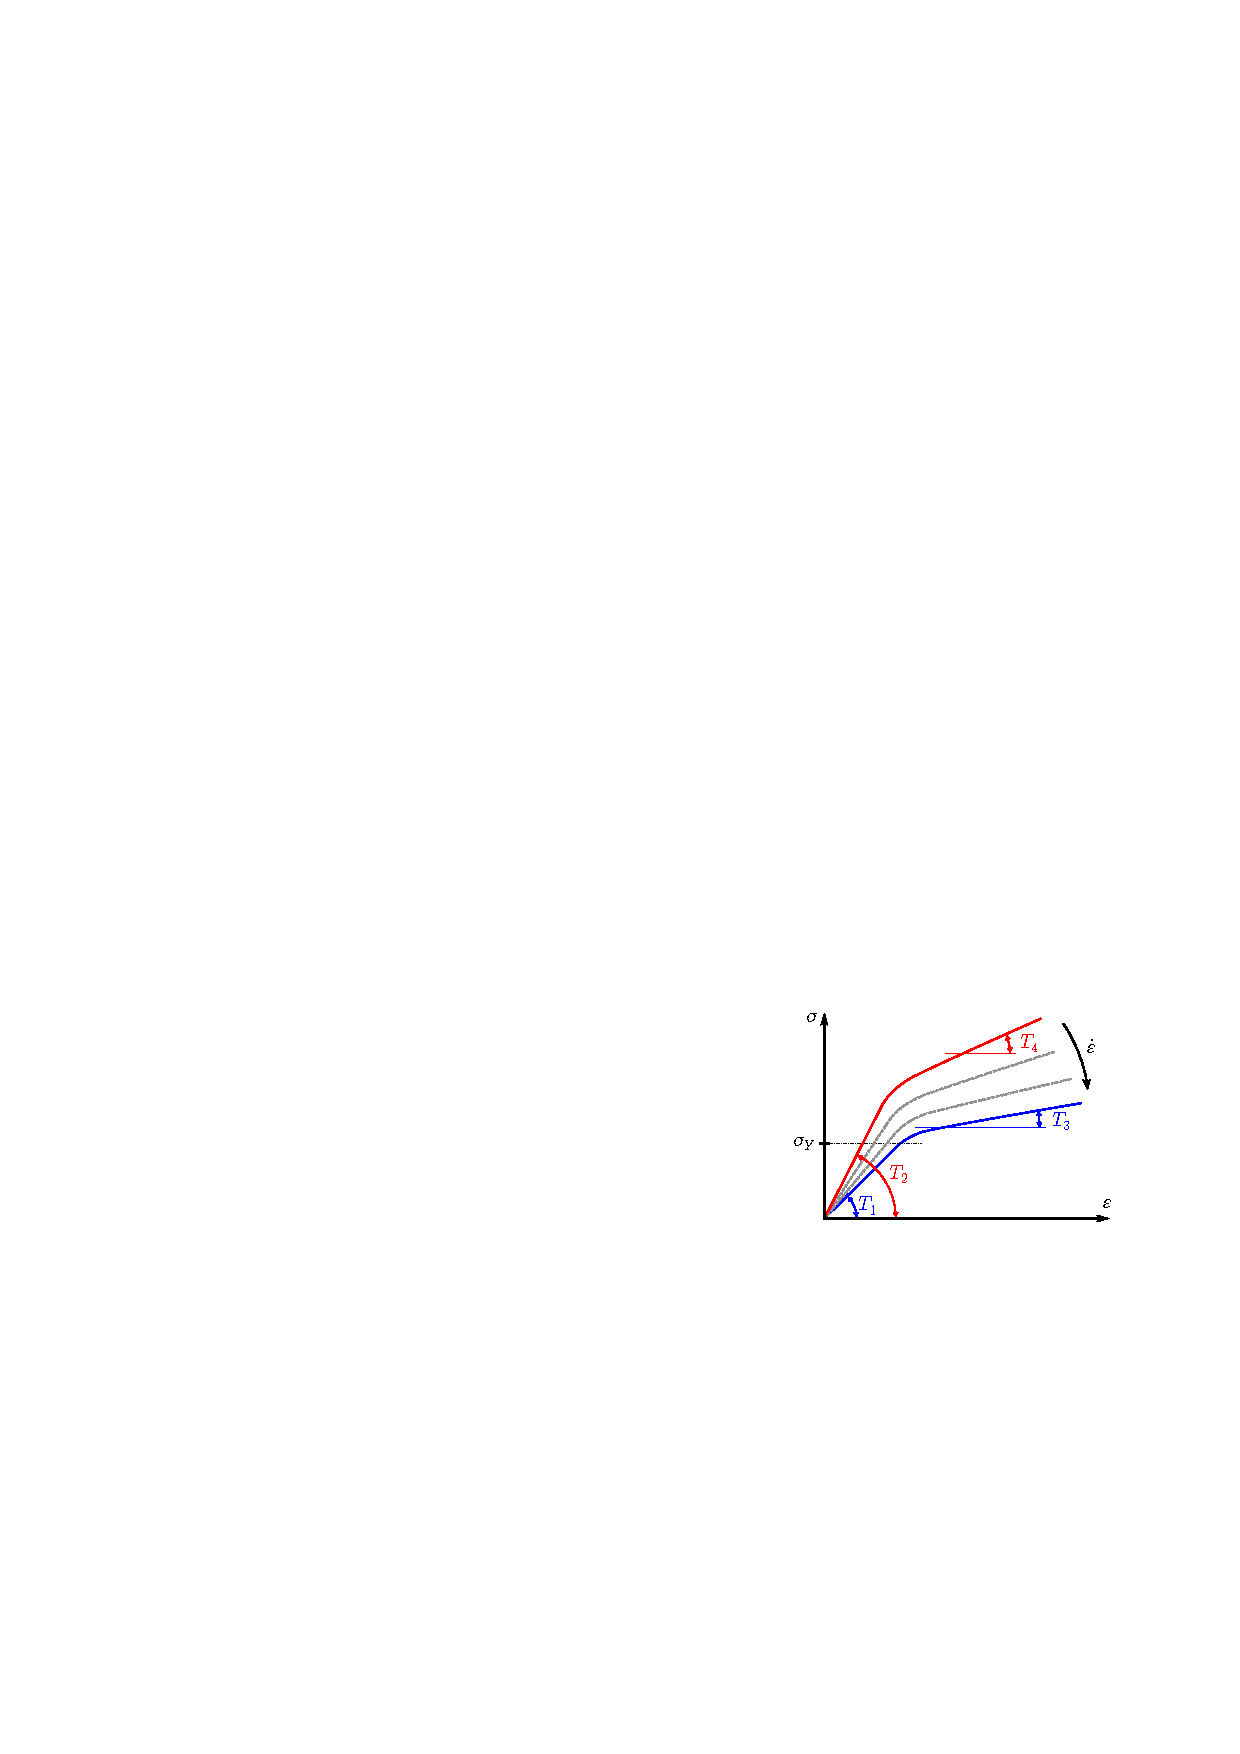
\includegraphics[scale=0.95]{Figuras/PTFE/calibration0.pdf} 
		
		\columnbreak
		
		\footnotesize
		\raggedright
		
		\textbf{1)} $T_1 \approx \young\indve \rightarrow $ Estima-se $\young\indve$ 
		
		\vspace{0.35cm}
		
		\textbf{2)} $T_2 \approx \young\indve + \young\inde \rightarrow $ Estima-se $\young\inde$ 
		
		\vspace{0.35cm}
		
		\textbf{3)} $T_3 \approx \dfrac{3\young\indve\armstrongstiff}{2\young\indve+2\armstrongstiff} \rightarrow $ Estima-se $\armstrongstiff$ 
		
		\vspace{0.35cm}
		
		\textbf{4)} $T_4 \approx \dfrac{3(\young\indve+\young\inde)(\armstrongstiff+\kinematicviscstiff)}{2\young\indve+2\young\inde+2\armstrongstiff+2\kinematicviscstiff} \rightarrow $ Estima-se $\kinematicviscstiff$ 
	\end{multicols}
	%\caption*{\textbf{Fonte:} Elaborado pelo autor}
\end{figure}

Novamente, os valores finais de rigidez plástica, bem como os parâmetros $\armstrongvisc$, $\visccin$, $\viscplast$ e $\overstresscte$, são calibrados manualmente. O parâmetro $\armstrongvisc$ está associado à evolução da rigidez plástica com o nível de deformação, e pode ser calibrado utilizando apenas o gráfico com menor taxa. Já a constante $\visccin$ está associada à variação da rigidez plástica com relação às taxas de deformação, e as constantes $\viscplast$ e $\overstresscte$ estão associadas à abertura da curva de transição entre os regimes viscoelásticos e viscoplásticos.

Os parâmetros calibrados são apresentados na \autoref{tab:parametros-PTFE}, sendo mostrados na \autoref{fig:calibracao-PTFE} os gráficos comparativos do modelo experimental com o numérico calibrado. Nesse, apresentam-se os valores de deformação linear de engenharia por tensão nominal (ou tensão de engenharia), sendo essa última calculada neste caso pela expressão $\bar{\cauchyind}_{11} = {\J}\cauchyind_{11}/{\Find_{11}} = \Find_{11}\Sind_{11}$. Como é possível observar, o modelo apresentado foi capaz de representar satisfatoriamente o comportamento dos gráficos em diferentes taxas de deformação, com exceção das transições entre os trechos viscoelásticos e viscoplásticos nos casos de maiores taxas, onde não foi possível acomodar a abertura das curvas numéricas com as experimentais, indicando uma possibilidade de melhoria no modelo viscoplástico.

\begin{table}[!htb]
	\centering
	\caption{parâmetros do modelo viscoelástico-viscoplástico calibrados para o material politetrafluoretileno}
	\footnotesize
	\label{tab:parametros-PTFE}
	{\renewcommand{\arraystretch}{1.1}
	\begin{tabular}{C{2.2cm} C{2.1cm} C{2.1cm} C{2.2cm}}
		\hline
		\rowcolor{LightGray}
		\multicolumn{4}{c}{Parâmetros viscoelásticos}  \\ \hline
		$\lame$ (MPa) & $\Gve$ (MPa) & $\Ge$ (MPa) & $\visc$ (MPa$\cdot$s)  \\  
		$1866.89$ & $97.98$ & $64.2614$ & $172.37$  \\
	\end{tabular}
	\begin{tabular}{C{1.9cm} C{1.8cm} C{0.5cm} C{1.8cm} C{2.2cm} C{1.5cm} C{1.6cm}}
		\hline
		\rowcolor{LightGray}
		\multicolumn{7}{c}{Parâmetros viscoplásticos}  \\ \hline
		$\yieldStresscte$ (MPa) & $\armstrongstiff$ (MPa) & $b$ & $\kinematicviscstiff$  (MPa) & $\visccin$ (MPa$\cdot$s) & $\viscplast$ (s) & $\overstresscte$ (MPa) \\ 
		$2.41$ & $51.71$ & $4$ & $8.27$ & $172.37$ & $9\cdot 10^6$ & $2$ \\ \hline
	\end{tabular}
	}
	%\caption*{\textbf{Fonte:} Elaborado pelo autor}
\end{table}

\begin{figure}[!htb]
	\centering
	\caption{Comparação entre resultados experimentais e numéricos para o ensaio de carregamento monotônico em material politetrafluoretileno}
	\label{fig:calibracao-PTFE}
	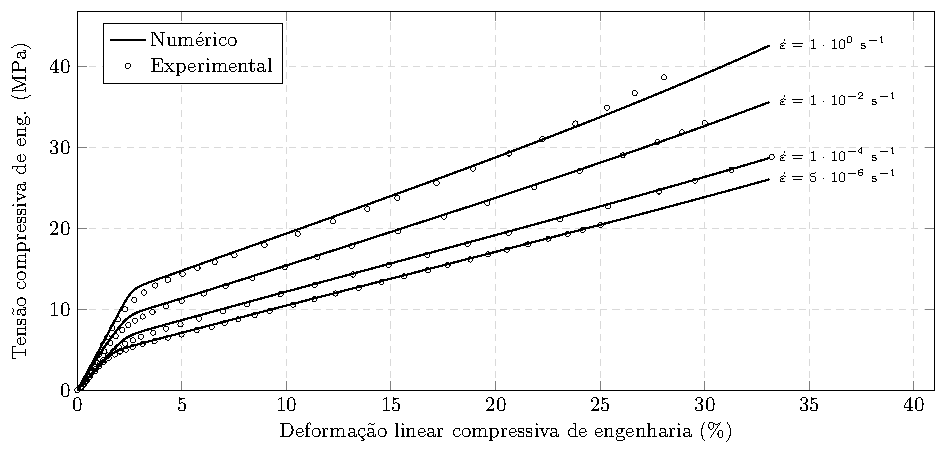
\includegraphics[scale=1.0]{Figuras/PTFE/khan-calibration.pdf}		
	%\caption*{\textbf{Fonte:} Elaborado pelo autor}
\end{figure}

Adicionalmente, para demonstrar a influência da parcela de encruamento cinemático viscoso na representação do comportamento constitutivo, apresenta-se na \autoref{fig:calibracao-PTFE-2} os resultados do ensaio de carregamento monotônico para $\kinematicviscstiff=0$. Dois casos são considerados: no primeiro, o valor de $\armstrongstiff$ é mantido igual ao original ($51,71$ MPa), e no segundo ele é tomado como a soma dos valores originais de $\armstrongstiff$ e $\kinematicviscstiff$ ($59,98$ MPa). Em ambos os casos, nota-se que a resposta numérica não condiz com o comportamento esperado, indicando que o modelo de Armstrong-Frederick não é capaz de representar isoladamente a dependência temporal da rigidez plástica. De fato, pode ser observado que, em cada caso, a rigidez plástica é aproximadamente a mesma para todas as taxas de deformação, adaptando-se apenas às menores taxas no primeiro caso, e às maiores taxas no segundo. Esses resultados sugerem que um componente viscoso de encruamento cinemático, ou qualquer formulação com efeito equivalente, é necessária para simular a resposta constitutiva do PTFE.

\begin{figure}[!htb]
	\centering
	\caption{Comparação entre resultados experimentais e numéricos para o ensaio de carregamento monotônico, desconsiderando o encruamento cinemático viscoso (isto é, $\kinematicviscstiff=0$), com (a) $\armstrongstiff = 51,71$ MPa e (b) $\armstrongstiff = 59,98$ MPa}
	\label{fig:calibracao-PTFE-2}
	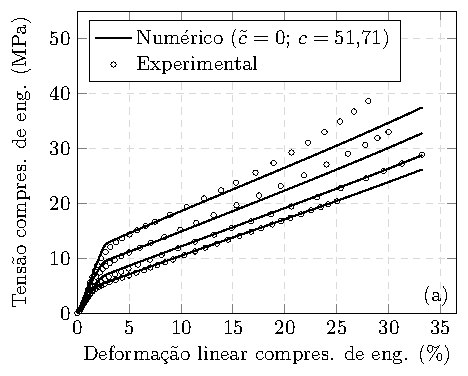
\includegraphics[scale=1.0]{Figuras/PTFE/khan-calibration-noViscousHardening1.pdf}\;\;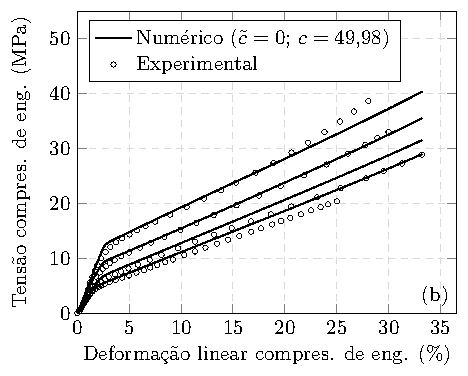
\includegraphics[scale=1.0]{Figuras/PTFE/khan-calibration-noViscousHardening2.pdf}		
	%\caption*{\textbf{Fonte:} Elaborado pelo autor}
\end{figure}

Neste mesmo exemplo, considerando os parâmetros originais, realiza-se uma análise da propriedade da conservação do volume inelástico. Na \autoref{fig:jacobian-analysis} são mostrados os erros dos jacobianos $\Jv$, $\Jp$, $\Jpi$ e $\Jpvi$ para as $4$ diferentes taxas de deformação, com $5$ diferentes valores de $\Delta t$. As inclinações das retas são, em todos os casos, próximas de $1$, indicando convergência de primeira ordem. Dessa forma, o erro dos Jacobianos, causado pelo algoritmo de retorno de Euler conforme discutido na \autoref{sec:solucao-numerica}, pode ser reduzido pela metade ao dobrar o número de passos de tempo. É interessante observar que, para os casos com menores taxas de deformação, os erros de $\Jpvi$ se tornam praticamente iguais aos de $\Jp$, uma vez que a parcela viscosa de deformação plástica tende a se comportar de forma equivalente à parcela plástica em intervalos de tempo muito longos.

\begin{figure}[!h]
	\centering
	\caption{Análise do Jacobiano}
	\label{fig:jacobian-analysis}
	\includegraphics[scale=1.0]{Figuras/PTFE/Jacobian-analysis.pdf}		
	%\caption*{\textbf{Fonte:} Elaborado pelo autor}
\end{figure}

\subsection{Ensaio de relaxação}\label{subsec:ptfe-relaxation}

O ensaio de relaxação apresentado em \citeonline{khan2001} é realizado em três etapas de carregamento, intercaladas por duas etapas de intervalo, e seguida de uma etapa de descarregamento. A taxa de deformação aplicada é $0,01$s$^{-1}$, tanto nas etapas de carregamento quanto na de descarregamento. Nas etapas de intervalo, as deformações são mantidas fixas por $6$h, nos valores de $0,0832$ e $0,1832$ para o primeiro e segundo intervalo, respectivamente. Para a solução numérica, consideram-se $4200$ passos de tempo, sendo $300$ para cada etapa de carregamento/descarregamento, e $1500$ para cada etapa de intervalo. Dessa forma, o valor de $\Delta t$ é variável ao longo da análise.

Na \autoref{fig:ptfe-relaxation} são mostrados os resultados dessa análise, e a comparação com a resposta experimental. Nota-se, em geral, uma boa concordância, especialmente para a primeira curva de relaxação da \autoref{fig:ptfe-relaxation}(b), onde as respostas são praticamente indistinguíveis. No entanto, a partir da segunda fase de carregamento, observa-se uma queda nos valores numéricos de tensão com relação aos experimentais. Esse problema pode ser atribuído à componente viscosa de encruamento cinemático, que continua evoluindo durante os intervalos, consequentemente reduzindo a rigidez plástica e a a tensão de escoamento. Para investigar esse efeito de forma mais aprofundada, também são incluídos na \autoref{fig:ptfe-relaxation} os resultados numéricos sem encruamento cinemático viscoso, considerando $\kinematicviscstiff=0$ e $\armstrongstiff = 60$ MPa. Verifica-se que, nesse caso, não há redução nos valores de tensão após os intervalos, e os resultados para o diagrama de tensão-deformação são excelentes. Apesar disso, é importante lembrar que o modelo sem encruamento cinemático viscoso é inconsistente com as demais taxas de deformação, sendo também inferior ao modelo original no diagrama de tensão ao longo do tempo.

\begin{figure}[!htb]
	\centering
	\caption{Gráficos de tensão compressiva de engenharia por (a) deformação linear compressiva de engenharia e (b) tempo, para o ensaio de relaxação com intervalos de $6$h e $\dot{\defLinearind}=0,01\,\text{s}^{-1}$.}
	\label{fig:ptfe-relaxation}
	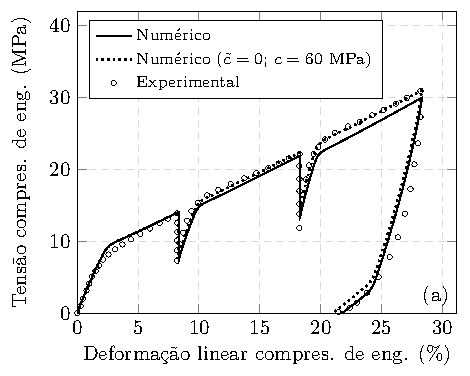
\includegraphics[scale=1.0]{Figuras/PTFE/Relaxation.pdf}\;\;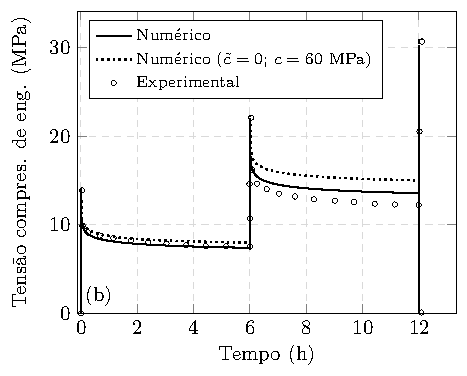
\includegraphics[scale=1.0]{Figuras/PTFE/Relaxation-s.pdf}		
	%\caption*{\textbf{Fonte:} Elaborado pelo autor}
\end{figure}

Em seguida, o mesmo exemplo é considerado utilizando diferentes taxas de deformação para cada etapa de carregamento e descarregamento. Os resultados numéricos dessa análise são mostrados na \autoref{fig:ptfe-relaxation-2}. Na \autoref{fig:ptfe-relaxation-2}(a) é possível ver que a redução no nível de tensão após cada intervalo de relaxação é notável apenas nos casos com maiores taxas, já que nesses há maior influência do encruamento cinemático viscoso. Com relação às curvas de relaxação, observa-se na \autoref{fig:ptfe-relaxation-2}(b) que os valores dos quatro casos tendem a convergir para o mesmo valor (tensão de escoamento), assumindo comportamentos bem similares entre si já na primeira hora de intervalo.

\begin{figure}[!htb]
	\centering
	\caption{Gráficos de tensão de engenharia por (a) deformação linear de engenharia e (b) tempo, para o ensaio de relaxação com intervalos de $6$h e taxas de deformação variáveis.}
	\label{fig:ptfe-relaxation-2}
	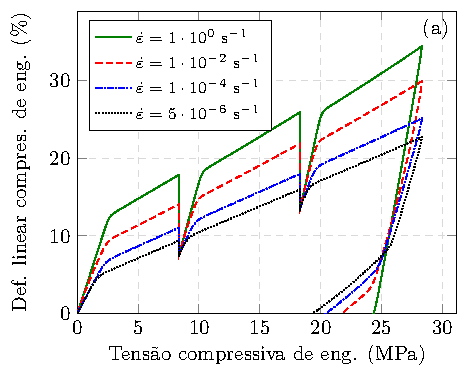
\includegraphics[scale=1.0]{Figuras/PTFE/Relaxation-all-rates.pdf}\;\;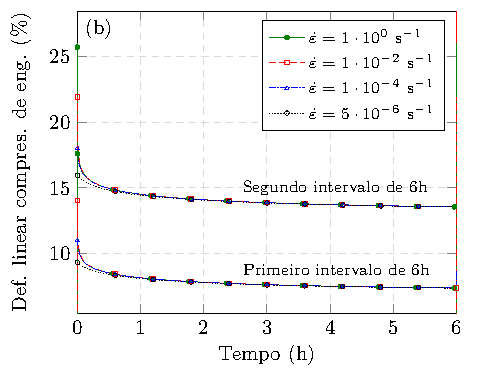
\includegraphics[scale=1.0]{Figuras/PTFE/Relaxation-all-rates-s-6h.pdf}		
	%\caption*{\textbf{Fonte:} Elaborado pelo autor}
\end{figure}

\subsection{Ensaio de fluência}\label{subsec:ptfe-creep}

Neste caso, ao invés de deformação prescrita, aplica-se tensão de engenharia prescrita (ou força distribuída). Novamente, consideram-se três etapas de carregamento, cada uma seguida por uma etapa de intervalo, sendo utilizadas as mesmas discretizações temporais do exemplo anterior. Nas etapas de carregamento, aplica-se taxa de tensão de engenharia constante de $0,17557$ MPa/s. Nas etapas de intervalo, as tensões são mantidas fixas por $6$h, nos valores de $9,653$ MPa, $14,892$ MPa e $17,582$ MPa para o primeiro, segundo e terceiro intervalo, respectivamente. Os resultados numéricos são comparados com os experimentais na \autoref{fig:ptfe-creep}, onde novamente pode ser vista uma conformação satisfatória das curvas, levando em conta as incertezas associadas. Além disso, observa-se que os resultados numéricos para o caso com $\kinematicviscstiff=0$ são equivalentes ao modelo original, indicando que o componente de encruamento cinemático viscoso não possui papel importante neste caso em particular.

\begin{figure}[!htb]
	\centering
	\caption{Gráficos de (a) tensão-deformação e (b) deformação ao longo do tempo, para o ensaio de fluência com intervalos de $6$h e taxa de tensão de $0,1755$ MPa/s.}
	\label{fig:ptfe-creep}
	\includegraphics[scale=1.0]{Figuras/PTFE/creep.pdf}\;\;\includegraphics[scale=1.0]{Figuras/PTFE/creep-e.pdf}		
	%\caption*{\textbf{Fonte:} Elaborado pelo autor}
\end{figure}

Adicionalmente, na \autoref{fig:ptfe-creep-all-rates} são mostrados os resultados do ensaio de fluência considerando diferentes taxas de tensão durante as etapas de carregamento e descarregamento. Como esperado, o valor médio de deformação aumenta com a taxa de tensão. Para as curvas de fluência, embora as deformações tendam aproximadamente ao mesmo valor, observa-se que os trechos intermediários são mais distintos entre si quando comparados com as curvas de relaxação do exemplo anterior.

\begin{figure}[!htb]
	\centering
	\caption{Gráficos de (a) tensão-deformação e (b) deformação ao longo do tempo, para o ensaio de fluência com intervalos de $6$h e taxa de tensão variável.}
	\label{fig:ptfe-creep-all-rates}
	\includegraphics[scale=1.0]{Figuras/PTFE/creep-all-rates.pdf}\;\;\includegraphics[scale=1.0]{Figuras/PTFE/creep-all-rates-e.pdf}%\caption*{\textbf{Fonte:} Elaborado pelo autor}	
\end{figure}

\subsection{Cilindro parcialmente comprimido}\label{subsec:cilindro}

Neste exemplo, considera-se um corpo de prova cilíndrico com material PTFE, sujeito a compressão parcial em ambas as faces. Devido à simetria, apenas um oitavo da geometria é discretizada, com as devidas restrições aplicadas em cada eixo de simetria gerado, resultando no problema mostrado na \autoref{fig:vep-cylinder-data}. A seguir, este exemplo é simulado em diversas condições de malha, refinamento temporal e evolução de carregamento.

\begin{figure}[!htb]
	\centering
	\caption{Dados para o exemplo do cilindro parcialmente comprimido}
	\label{fig:vep-cylinder-data}
	{\small
		\noindent\shadowbox{
			\parbox{15.3cm}{
				\setlength{\columnseprule}{1pt}
				\vspace{-0.2cm}
				{\centering\begin{center}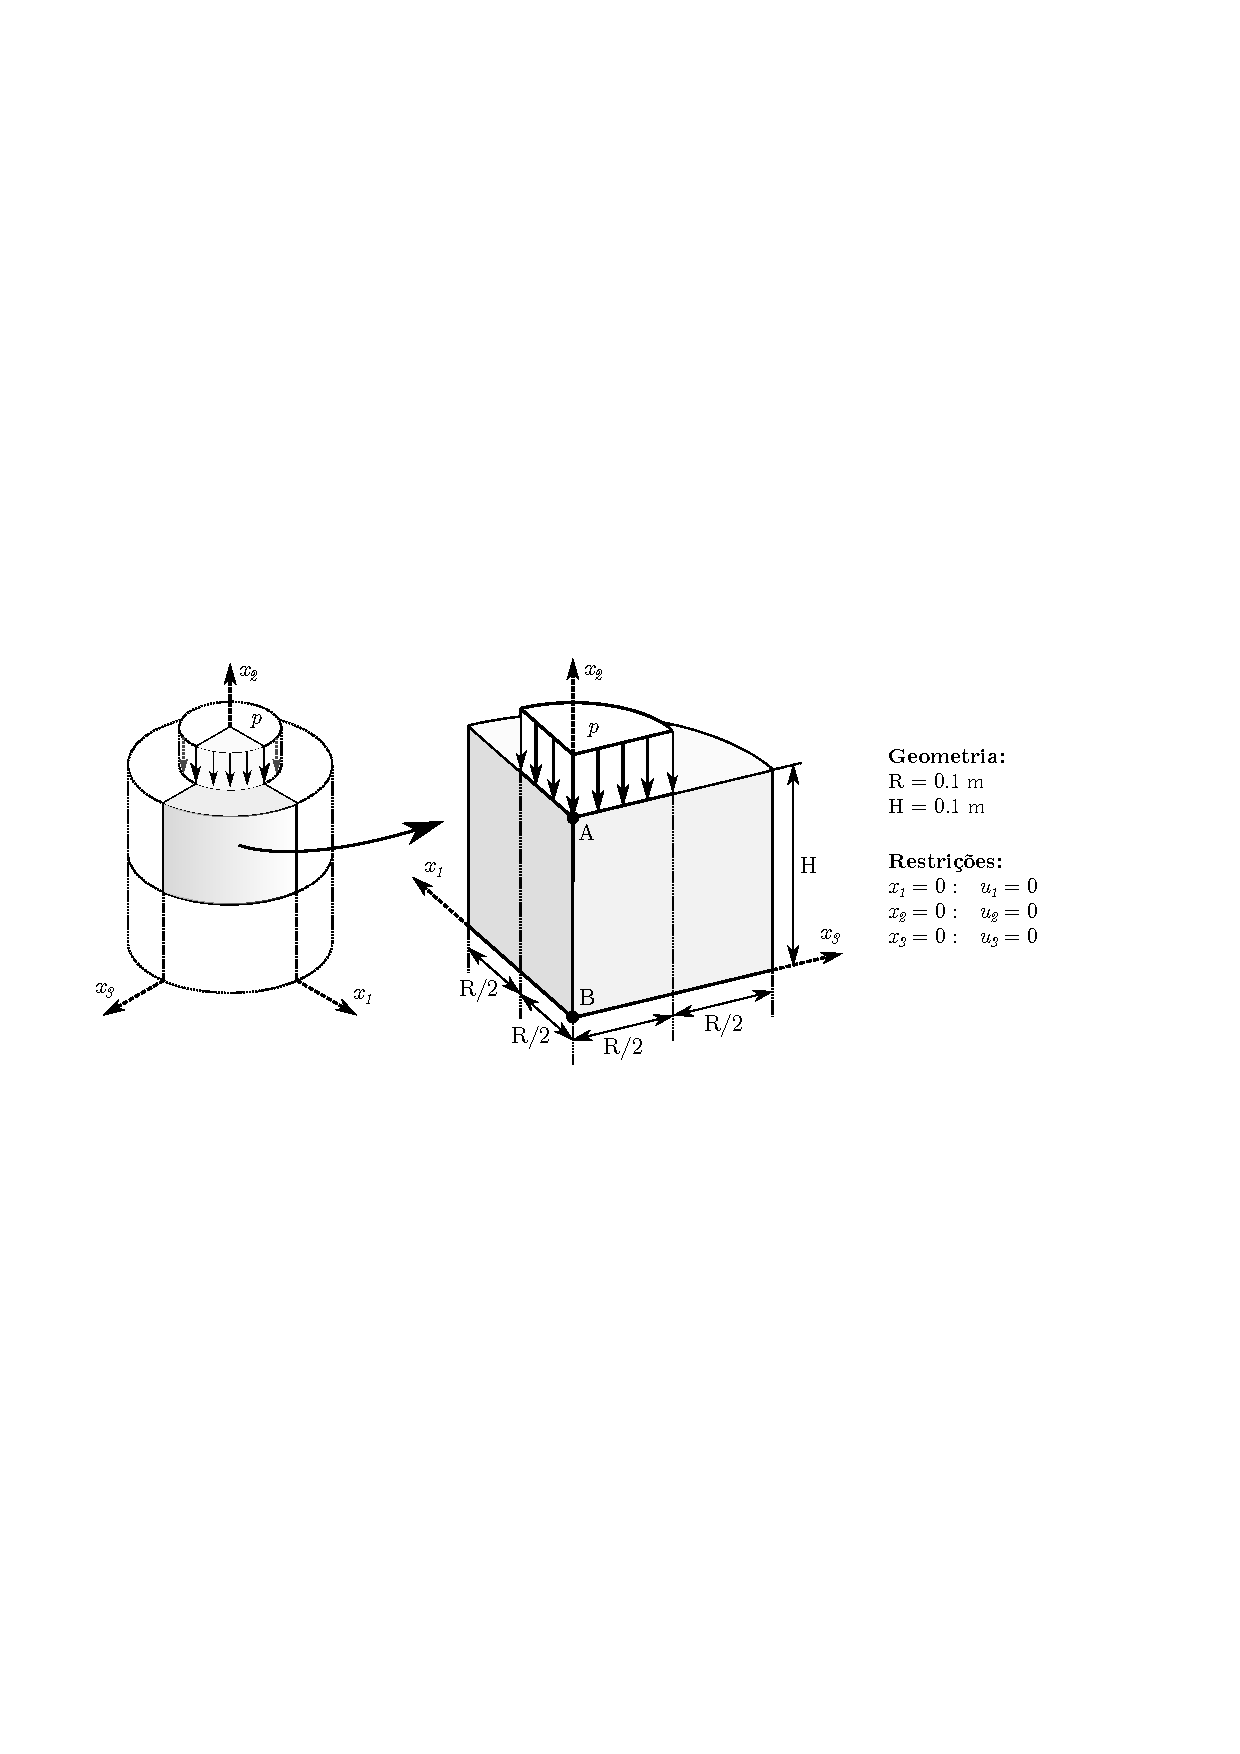
\includegraphics[scale=0.85]{Figuras/PTFE-cylinder-mesh/VepCylinder-data.pdf}	\end{center}\par}
				\vspace{-0.2cm}
			}
		}
	}	
	%\caption*{\textbf{Fonte:} Elaborado pelo autor}
\end{figure}


\subsubsection{Ensaio de fluência com análise de convergência de malha}

Nesta análise, considera-se que a força $p$ aplicada no cilindro possui valor $21$ MPa, fixo ao longo de um tempo total de $10^6$ s. Aqui, utiliza-se uma abordagem diferente para a discretização temporal: ao invés de intervalos de tempo fixos, os valores de $\Delta t$ evoluem conforme uma progressão geométrica. Essa abordagem é particularmente apropriada para exemplos com evolução do tipo logarítmica, uma vez que permite o uso de intervalos de tempo menores no início da análise, onde a taxa de deslocamento é maior, e intervalos de tempo maiores no final da análise, onde os resultados são relativamente estáveis, otimizando portanto o número total de passos necessário. Neste caso, aplicam-se 400 passos de tempo, com $\Delta t$ inicial de $1,28356$ s, e razão da progressão geométrica de $1,025$, resultando em um valor final de $2,43915\cdot 10^{4}$ s para o $\Delta t$.

Adotam-se, neste problema, elementos finitos hexaédricos (HEX8, HEX27 e HEX64) para discretizar o domínio do sólido. Ao total, utilizam-se $15$ malhas diferentes, sendo $5$ para cada tipo de elemento. Uma vez que o problema é radialmente simétrico, o refinamento é aplicado apenas nas interfaces transversais do cilindro, sendo utilizadas malhas com 2x2, 4x4, 8x8, 16x16 e 32x32 elementos transversais. O número de camadas radiais é mantida fixa para cada tipo de elemento, com valor apenas suficiente para representar adequadamente a geometria. Considerando a performance computacional, esse valor é tomado menor para os elementos de ordem maior, uma vez que esses contam com mais nós e, em geral, uma melhor interpolação.

Os deslocamentos verticais no ponto A para cada caso são apresentados na \autoref{fig:vep-cylinder-v}. A evolução ao longo do tempo é mostrada separadamente para os casos com elemento HEX8, HEX27 e HEX64, nas Figuras \ref{fig:vep-cylinder-v}(b), \ref{fig:vep-cylinder-v}(c) e \ref{fig:vep-cylinder-v}(d), respectivamente. Como pode ser visto, devido à alta não-linearidade do problema, os resultados são expressivamente dependentes da malha, sendo exigido um relativamente alto grau de refinamento para uma boa convergência dos gráficos, especialmente utilizando o elemento de ordem linear (HEX8), que sofre do efeito de \emph{locking}. Na \autoref{fig:vep-cylinder-v}(a), mostra-se ainda o erro do deslocamento máximo em cada caso, tomado com relação à malha mais refinada (HEX64/32x32). Nota-se que os casos com HEX27/32x32 e HEX64/16x16 apresentam resultados similares, com erro suficientemente pequeno em relação à malha de referência. A configuração deformada final para cada caso pode ser vista na \autoref{fig:vep-cylinder-deformed}.

\begin{figure}[!htb]
	\centering
	\caption{Deslocamentos verticais no ponto A para o cilindro parcialmente comprimido submetido à fluência, considerando (a) erro do deslocamento com relação à malha HEX64/32x32, e diagramas de deslocamento ao longo do tempo para os casos com elementos (b) HEX8, (c) HEX27 e (d) HEX64}
	\label{fig:vep-cylinder-v}
	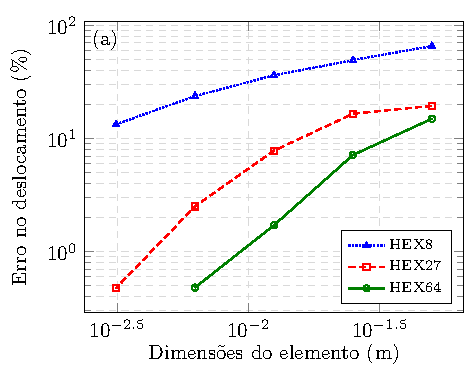
\includegraphics[scale=1.0]{Figuras/PTFE-cylinder-mesh/VepCylinder-Creep-v-Conv.pdf}\;\;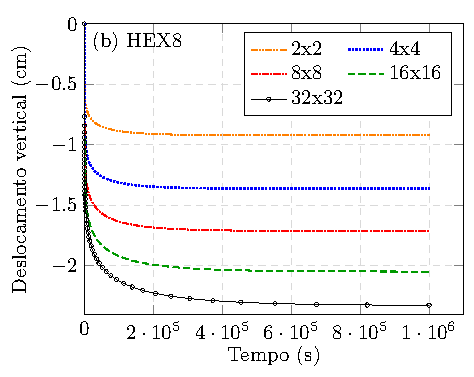
\includegraphics[scale=1.0]{Figuras/PTFE-cylinder-mesh/VepCylinder-Creep-v-1.pdf}	
	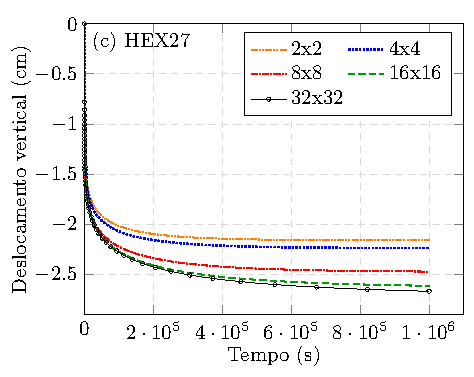
\includegraphics[scale=1.0]{Figuras/PTFE-cylinder-mesh/VepCylinder-Creep-v-2.pdf}\;\;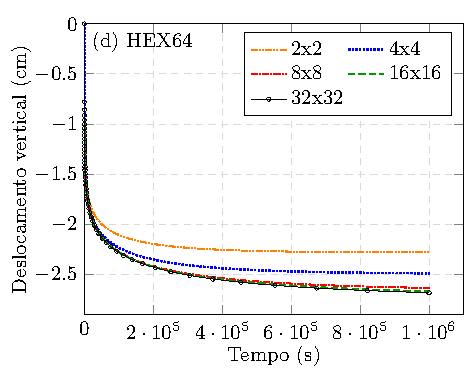
\includegraphics[scale=1.0]{Figuras/PTFE-cylinder-mesh/VepCylinder-Creep-v-3.pdf}		
	%\caption*{\textbf{Fonte:} Elaborado pelo autor}
\end{figure}

\begin{figure}[!htb]
	\centering
	\caption{Configurações deformadas para o cilindro parcialmente comprimido sob fluência em diferentes malhas, com componente $\left(\Epind\right)_{22}$ de deformação plástica em mapas de cores}
	\label{fig:vep-cylinder-deformed}
	\scriptsize HEX8 \hspace{4.2cm} HEX27 \hspace{4.2cm} HEX64 \hspace{0.7cm} \phantom{a}
	{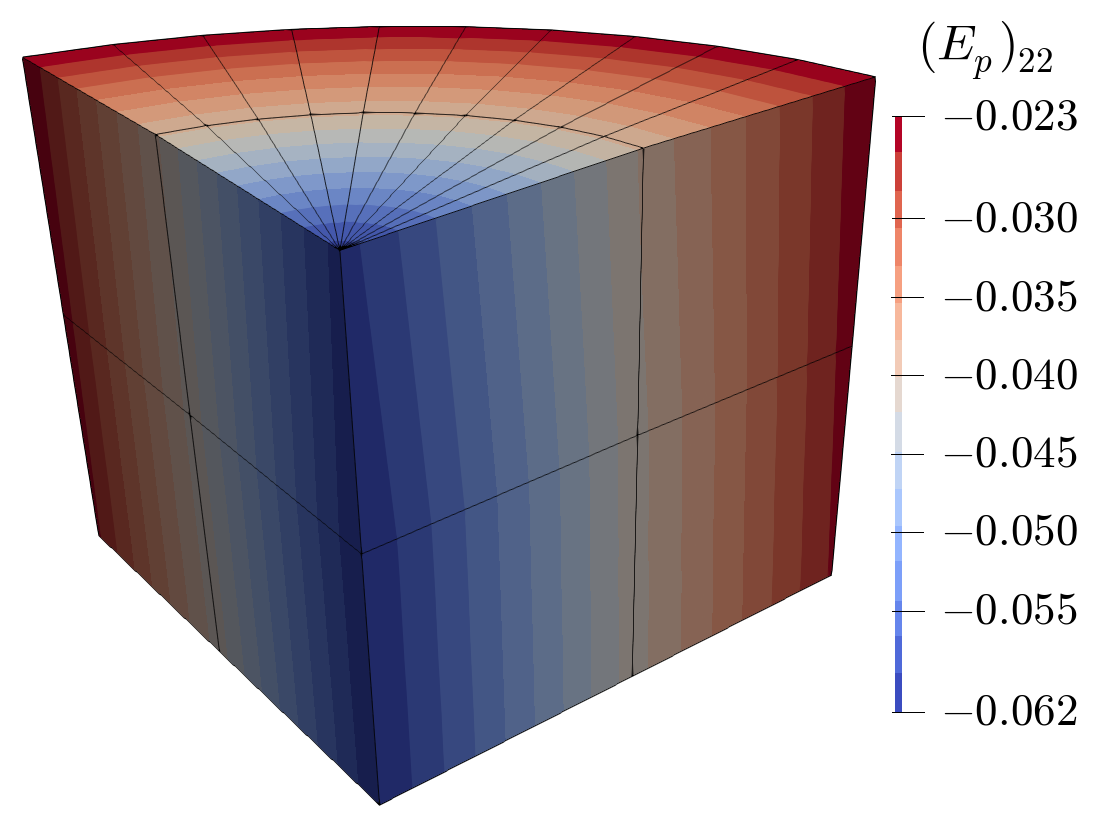
\includegraphics[scale=0.137]{Figuras/PTFE-cylinder-mesh/VepCylinder-2x2-1.png}}{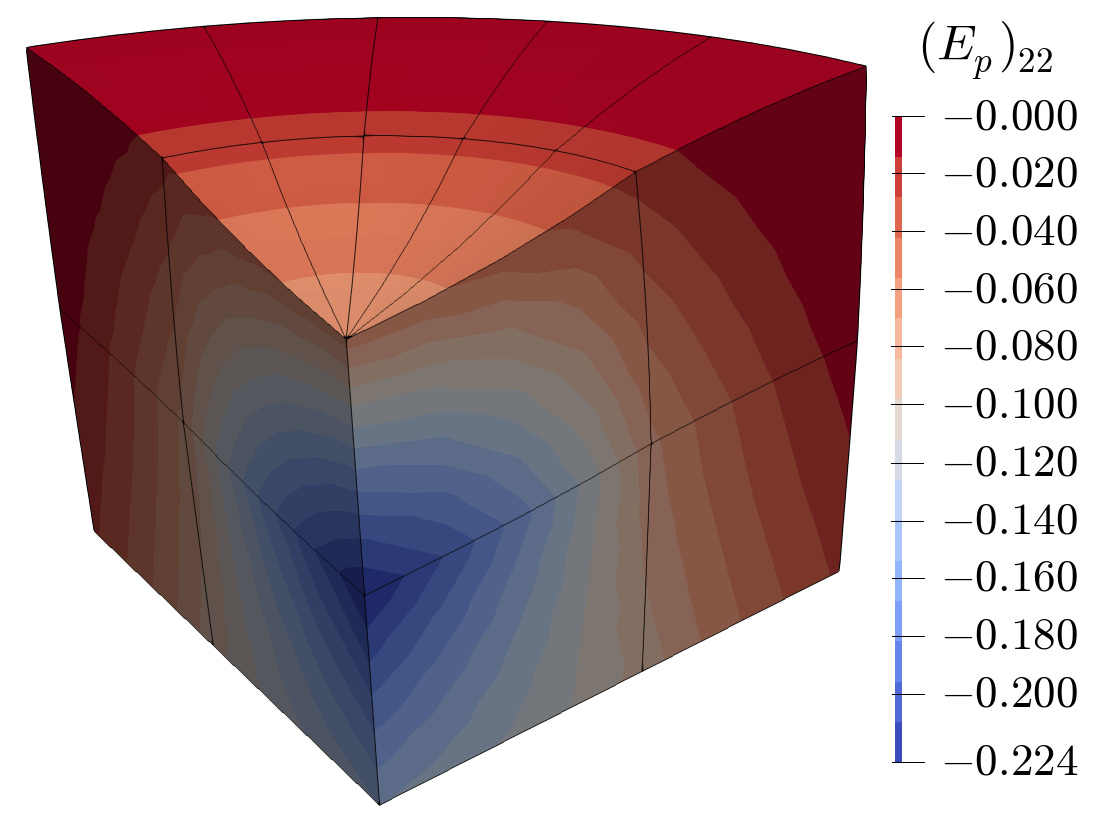
\includegraphics[scale=0.137]{Figuras/PTFE-cylinder-mesh/VepCylinder-2x2-2.png}}{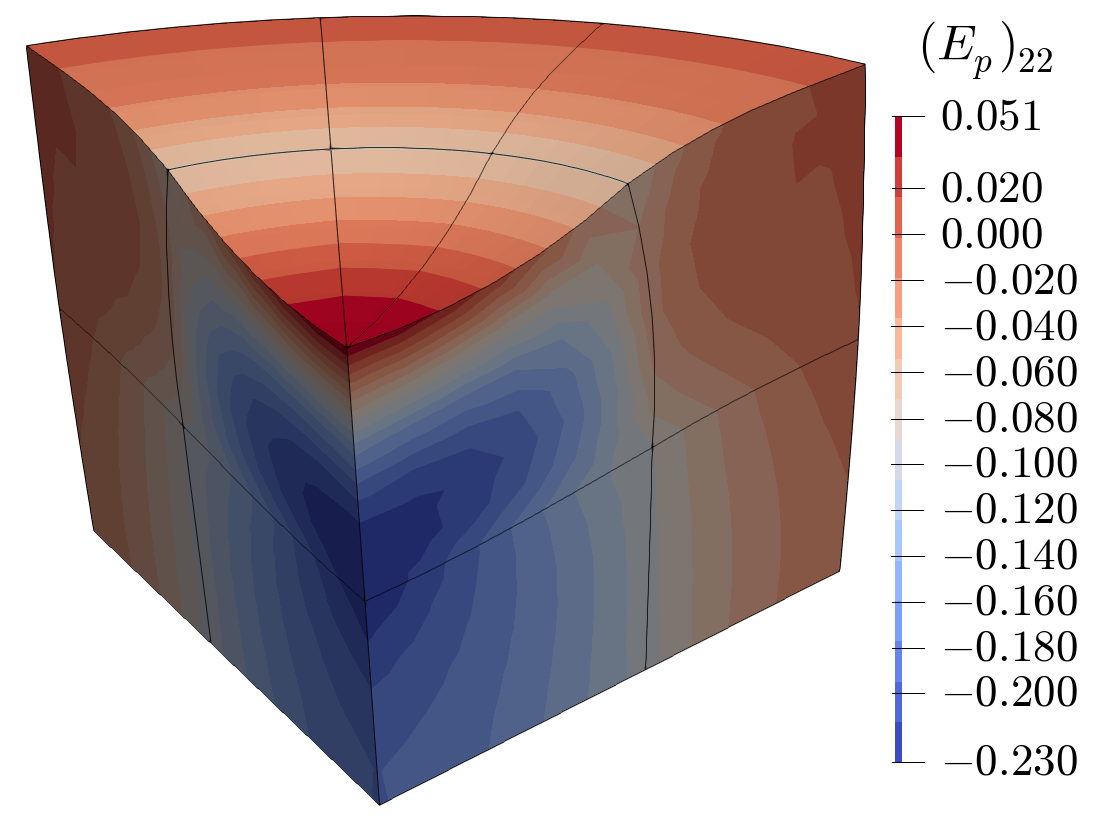
\includegraphics[scale=0.137]{Figuras/PTFE-cylinder-mesh/VepCylinder-2x2-3.png}}
	{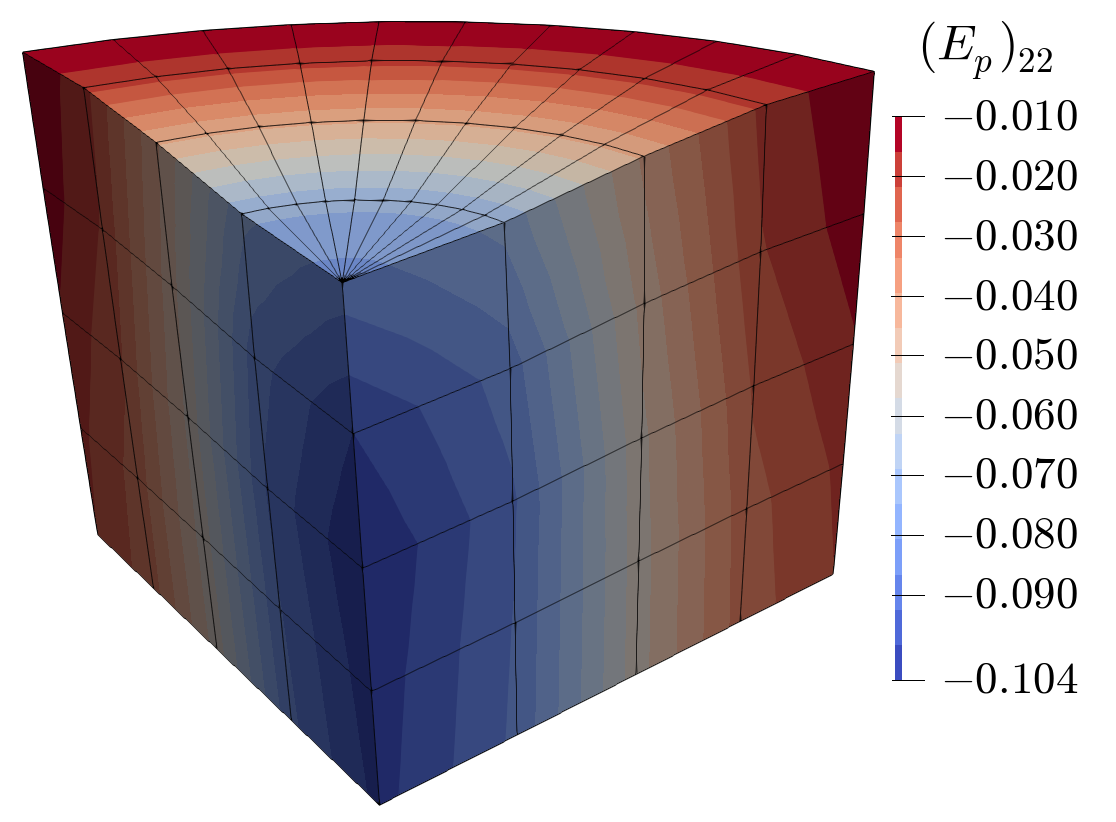
\includegraphics[scale=0.137]{Figuras/PTFE-cylinder-mesh/VepCylinder-4x4-1.png}}{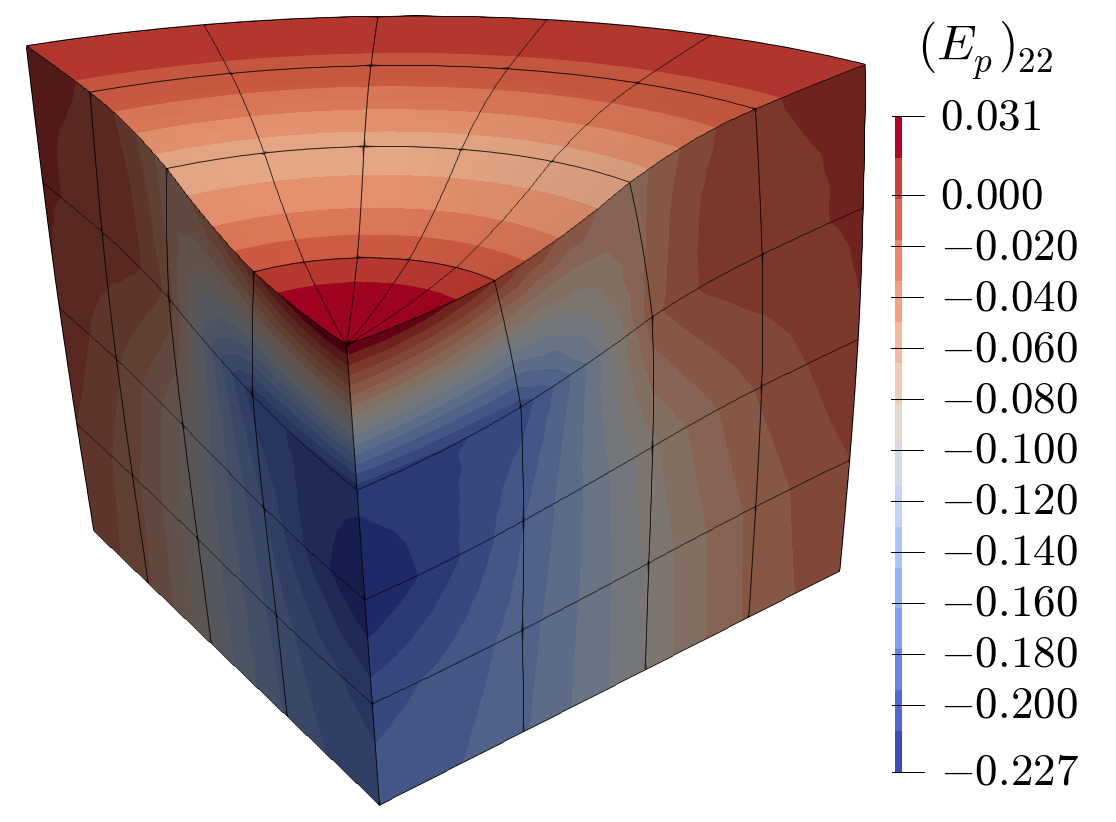
\includegraphics[scale=0.137]{Figuras/PTFE-cylinder-mesh/VepCylinder-4x4-2.png}}{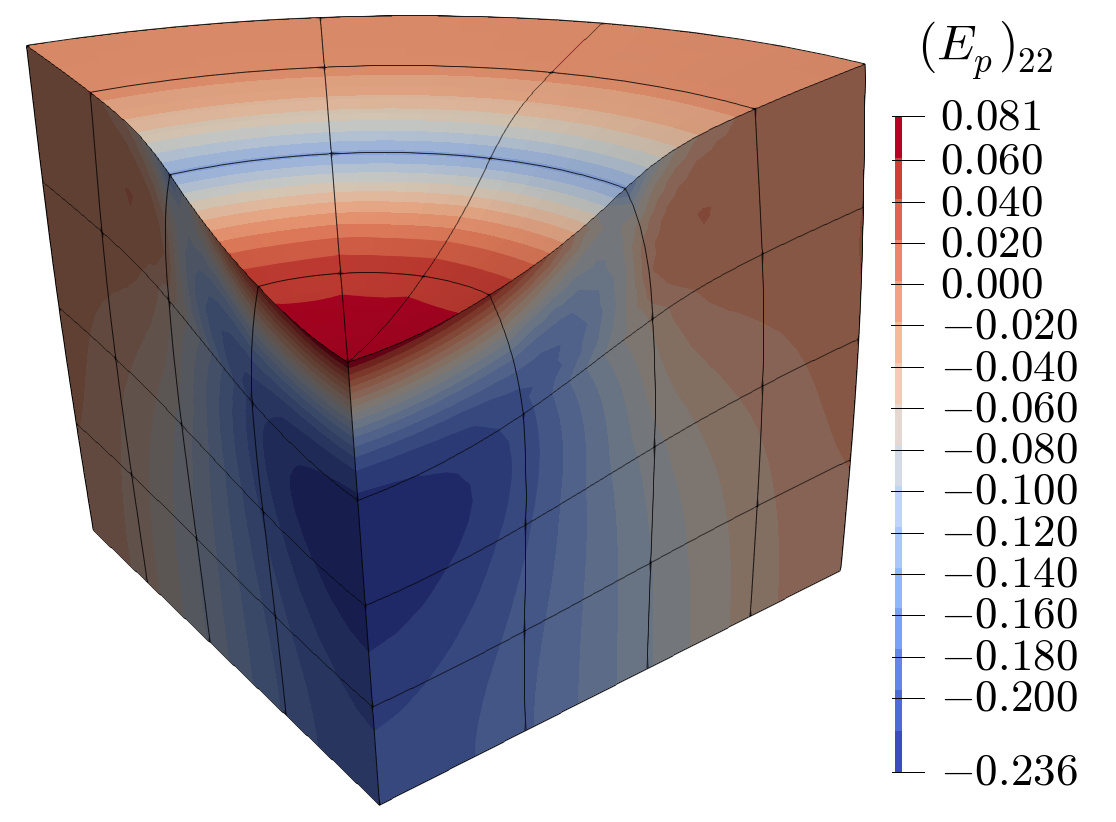
\includegraphics[scale=0.137]{Figuras/PTFE-cylinder-mesh/VepCylinder-4x4-3.png}}
	{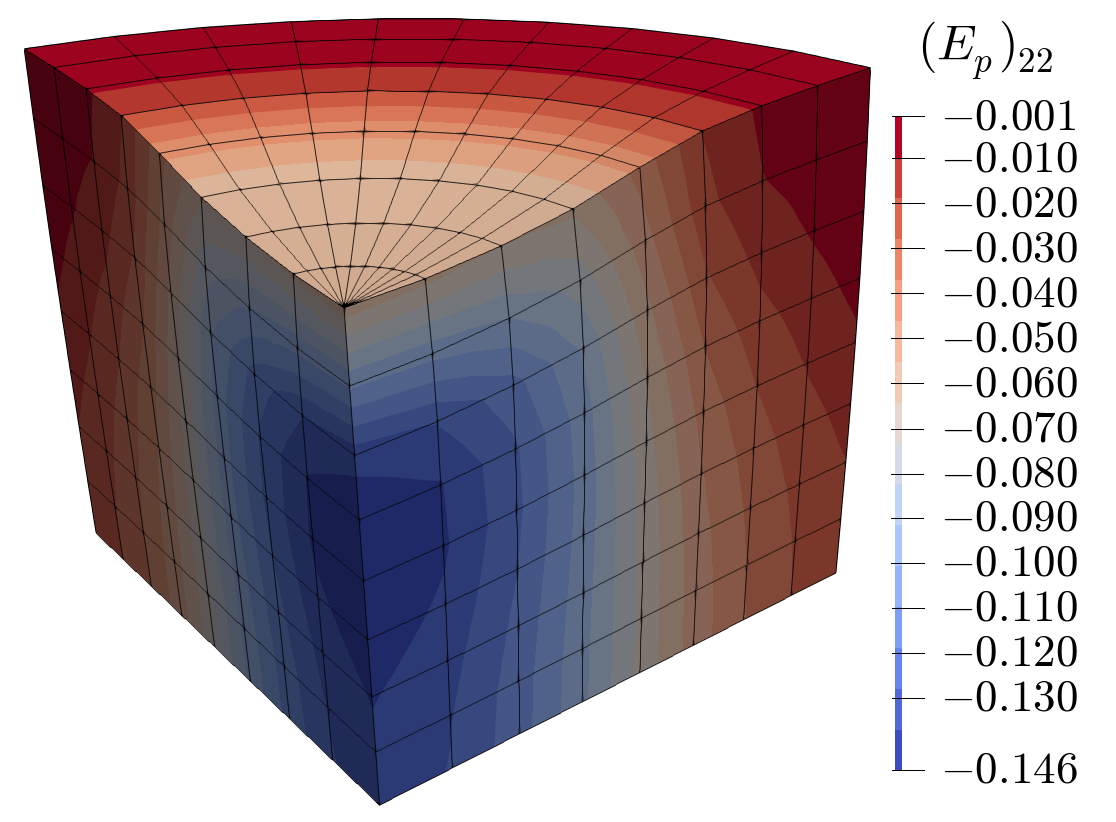
\includegraphics[scale=0.137]{Figuras/PTFE-cylinder-mesh/VepCylinder-8x8-1.png}}{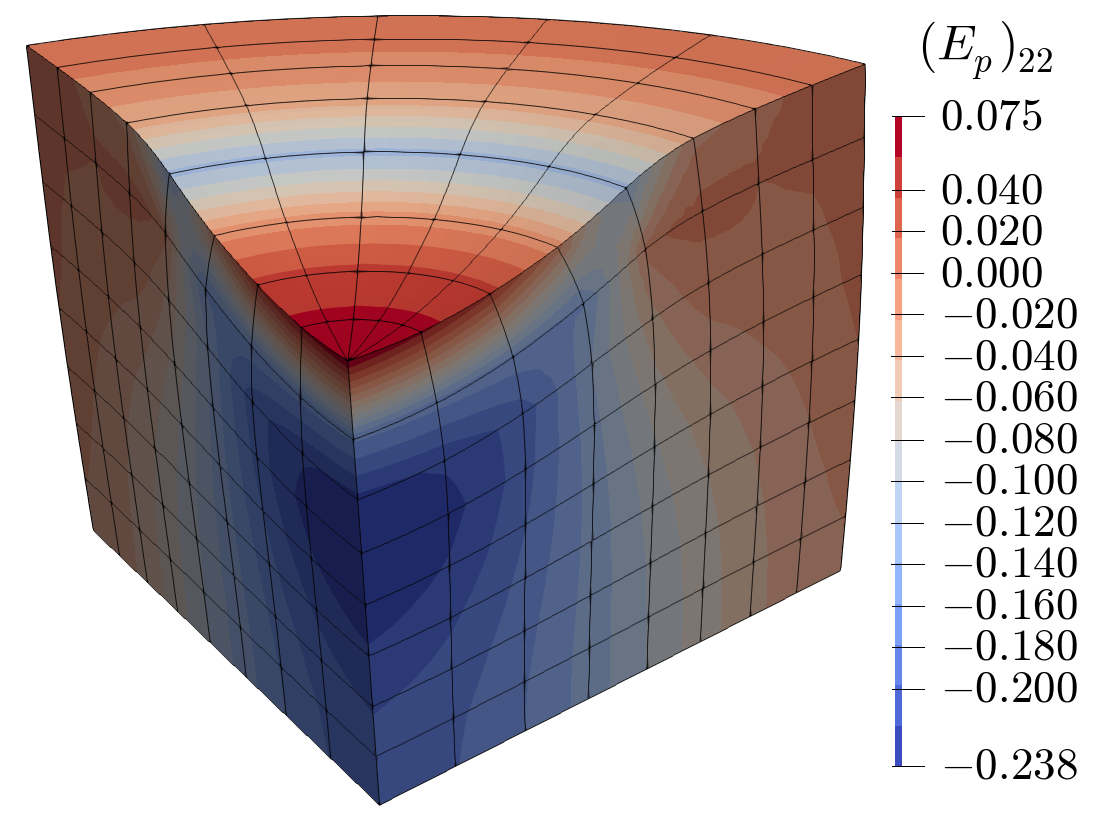
\includegraphics[scale=0.137]{Figuras/PTFE-cylinder-mesh/VepCylinder-8x8-2.png}}{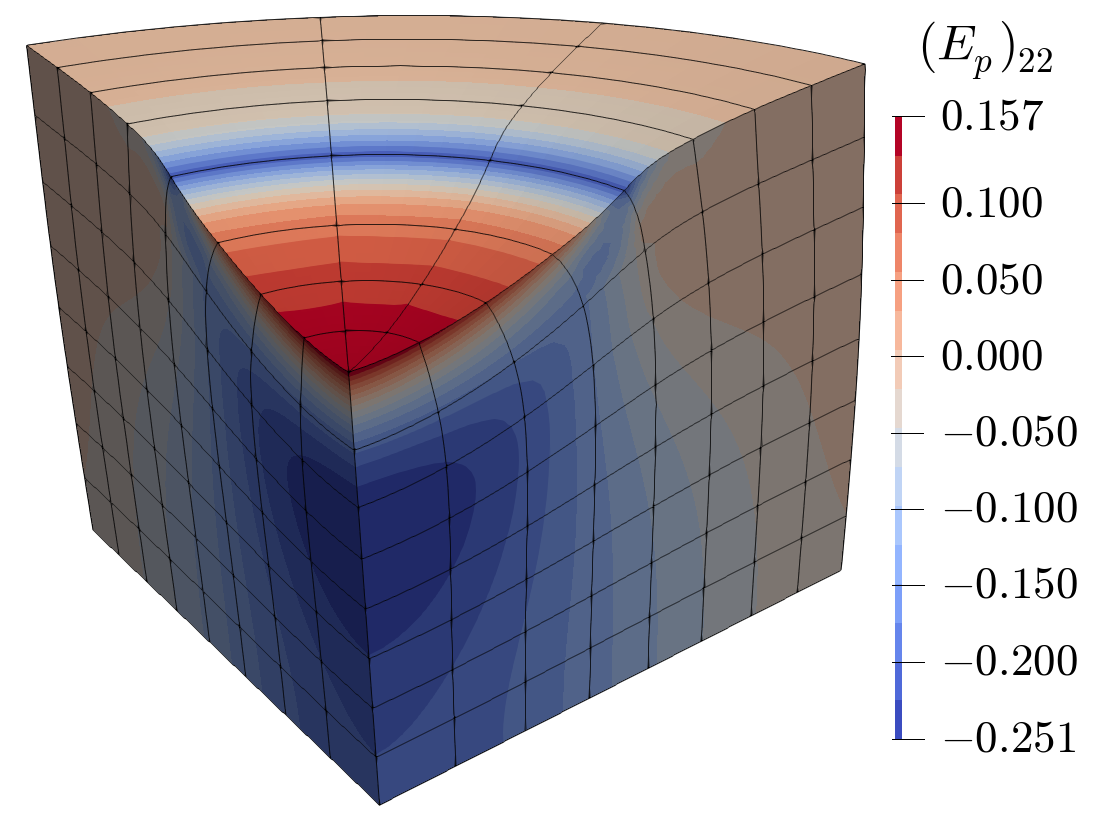
\includegraphics[scale=0.137]{Figuras/PTFE-cylinder-mesh/VepCylinder-8x8-3.png}}
	{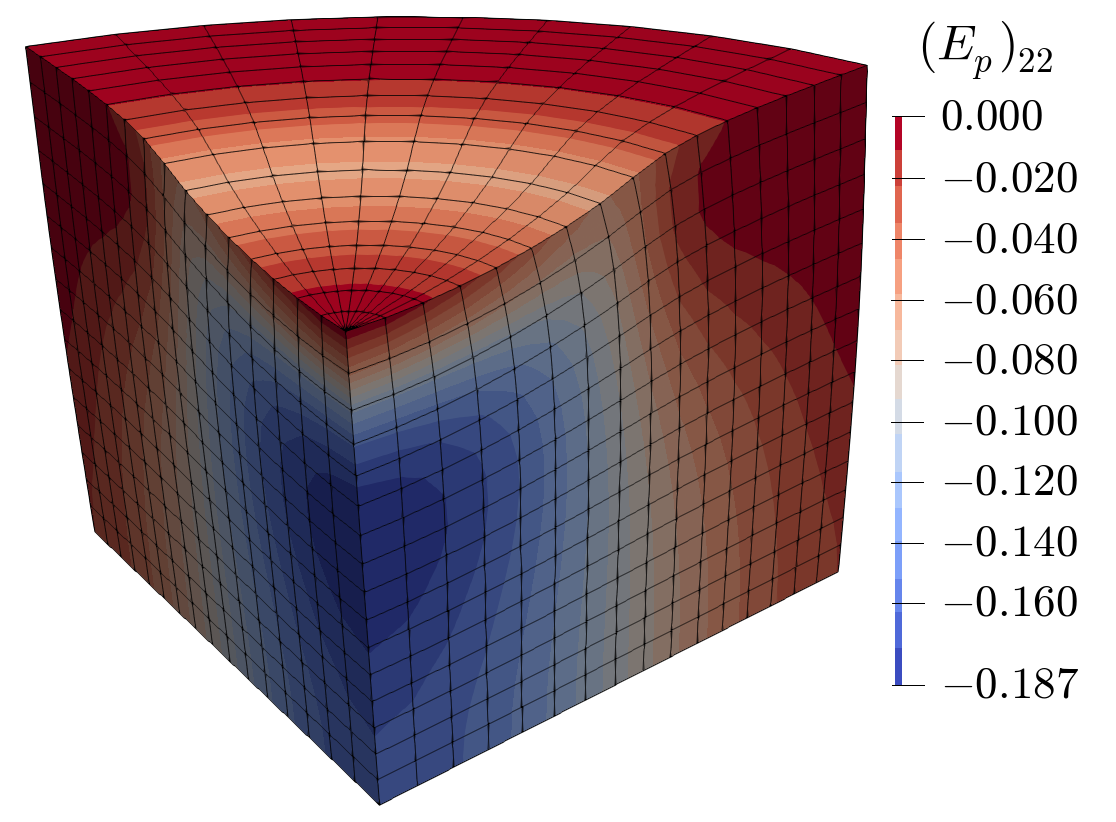
\includegraphics[scale=0.137]{Figuras/PTFE-cylinder-mesh/VepCylinder-16x16-1.png}}{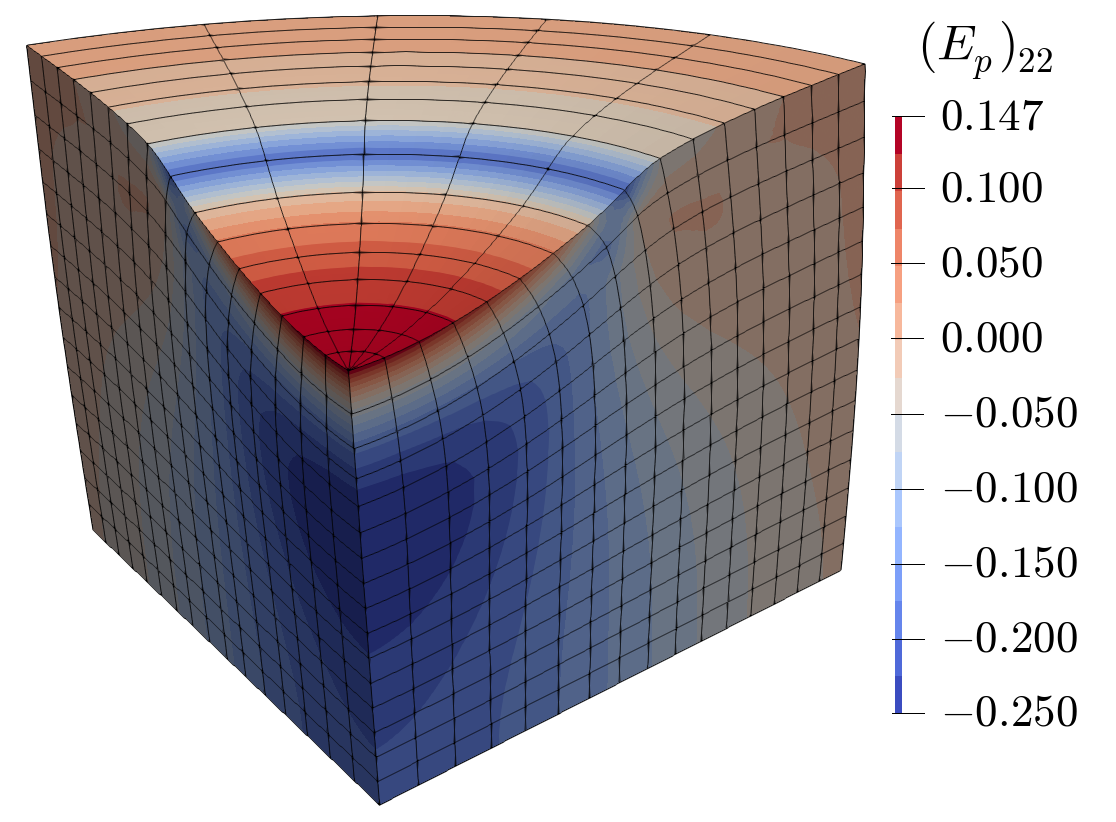
\includegraphics[scale=0.137]{Figuras/PTFE-cylinder-mesh/VepCylinder-16x16-2.png}}{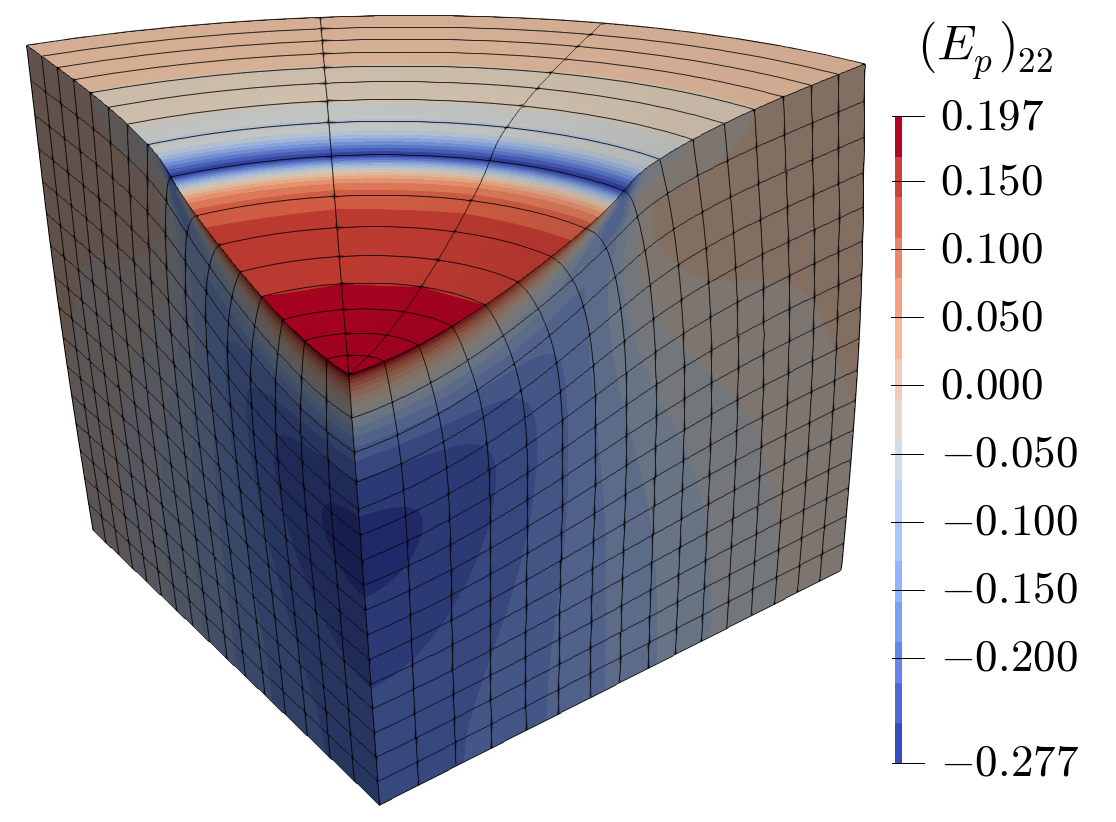
\includegraphics[scale=0.137]{Figuras/PTFE-cylinder-mesh/VepCylinder-16x16-3.png}}
	{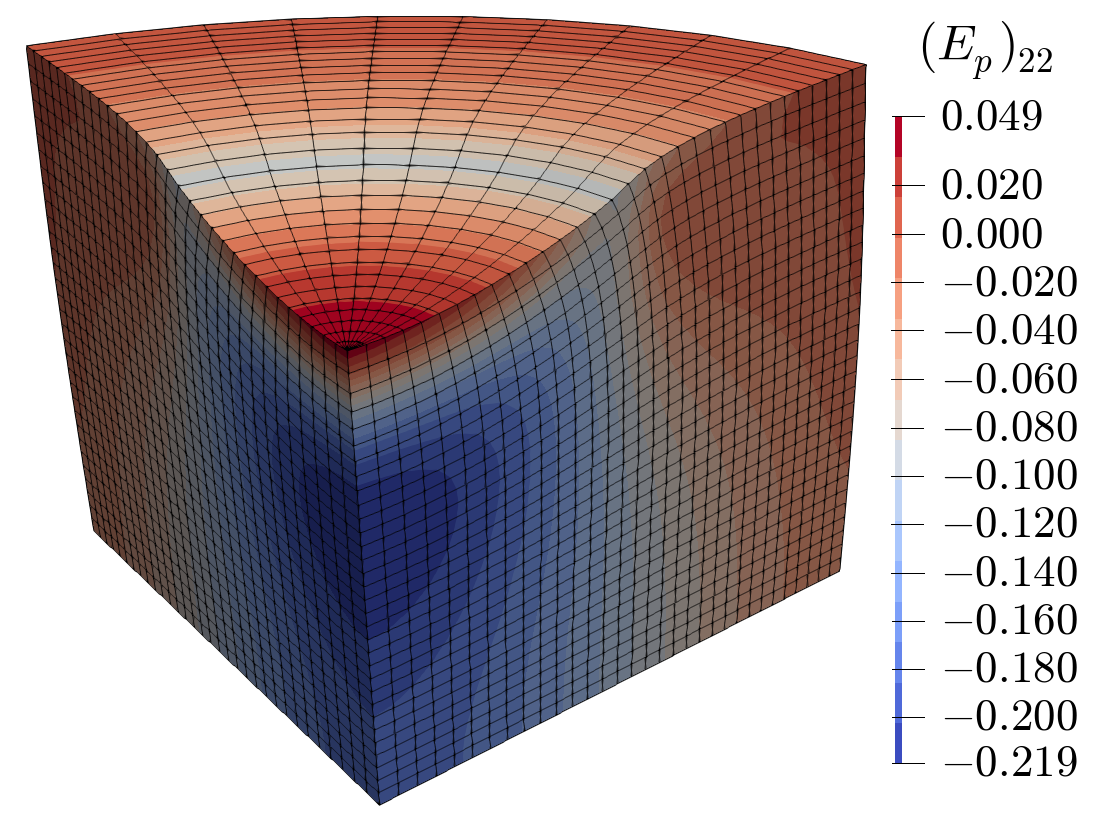
\includegraphics[scale=0.137]{Figuras/PTFE-cylinder-mesh/VepCylinder-32x32-1.png}}{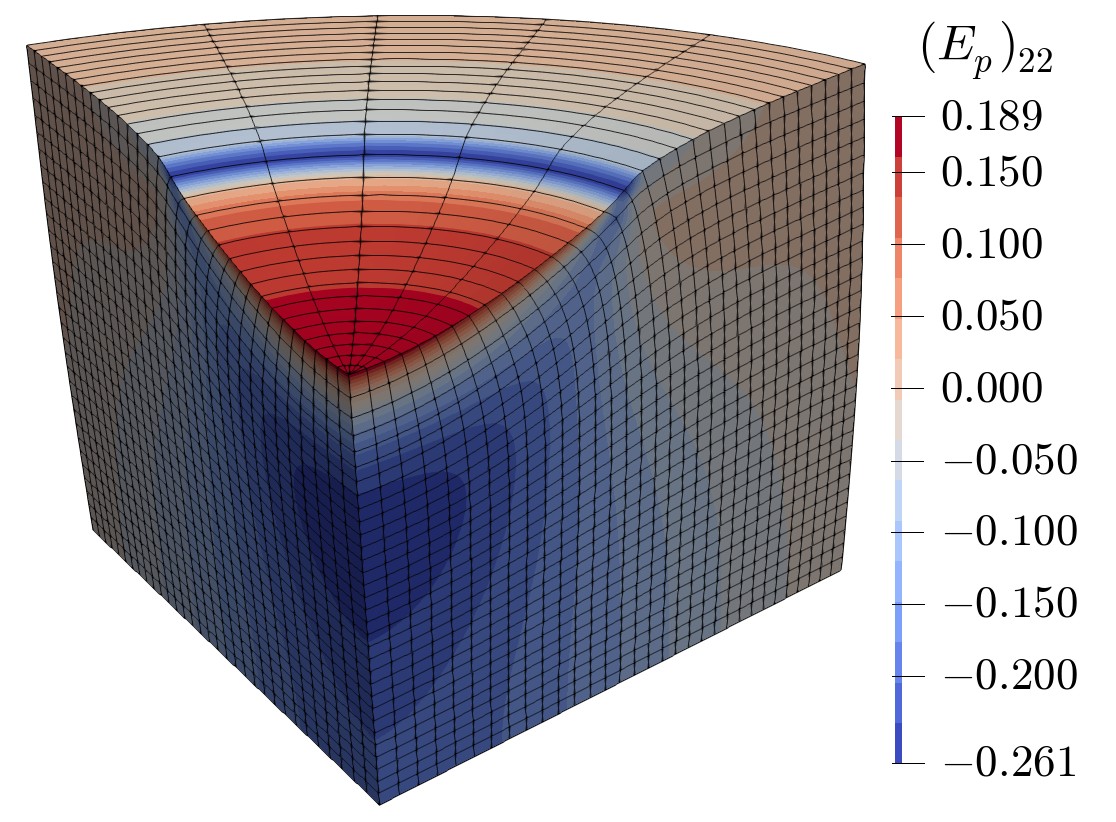
\includegraphics[scale=0.137]{Figuras/PTFE-cylinder-mesh/VepCylinder-32x32-2.png}}{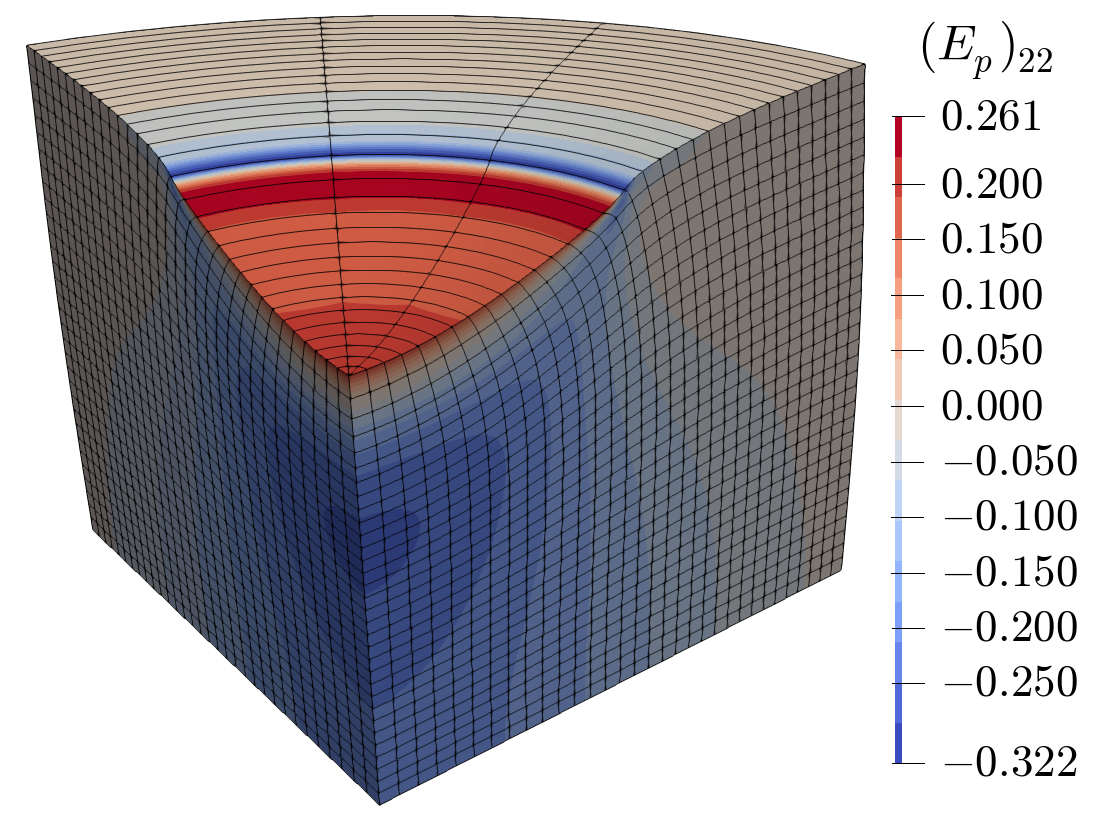
\includegraphics[scale=0.137]{Figuras/PTFE-cylinder-mesh/VepCylinder-32x32-3.png}}
	%\caption*{\textbf{Fonte:} Elaborado pelo autor}
\end{figure}

Os dados do problema relacionados à performance computacional são compilados na \autoref{tab:convergence-mesh} para cada malha considerada, sendo todos os casos executados no mesmo \emph{cluster} e sob condições equivalentes. O tempo de processamento em horas também pode ser visto em forma de gráfico na \cref{fig:cylinderCreep-conv}(a). Observa-se que a malha mais refinada (HEX64/32x32) possui um tempo de execução aproximadamente $5.1$ vezes maior do que a malha HEX27/32x32, e em torno de $6.9$ vezes maior do que a malha HEX64/16x16. Portanto, caso seja necessária uma boa precisão com custo computacional moderado, a malha HEX64/16x16 se torna mais vantajosa. No entanto, para situações práticas onde uma alta precisão não é necessária, a malha HEX64/8x8 também é uma opção adequada, com um tempo de processamento de aproximadamente $2.8\%$ em relação à mais refinada. Por outro lado, a malha HEX27/16x16 não é indicada, uma vez que ela possui um maior tempo de processamento e ainda maior erro quando comparada à HEX64/8x8.

\begin{table}[!h]
	\centering
	\scriptsize
	\caption{Análise de convergência de malha para o cilindro parcialmente comprimido sob fluência}
	\label{tab:convergence-mesh}
	{\renewcommand{\arraystretch}{1.2}
		\begin{tabular}{ccccccccc}
			\hline
			ORD & NSUB & NELEM & NGDL & DESLY (cm) & NITER & ITER-MED & TP (s) & TP-EF (s)\\ \hline
			\multirow{6}{*}{$1$} 
			& $2 $ & $   40$ & $   297$ & $-0.920576$ & $ 802$ & $2.005$ & $     33.3$ & $    32.5$ \\
			& $4 $ & $  160$ & $   825$ & $-1.361507$ & $ 857$ & $2.143$ & $    126.4$ & $   123.5$ \\
			& $8 $ & $  640$ & $  2673$ & $-1.711853$ & $1247$ & $3.118$ & $    681.1$ & $   670.3$ \\
			& $16$ & $ 2560$ & $  9537$ & $-2.046559$ & $1290$ & $3.225$ & $   2845.3$ & $  2802.5$ \\
			& $32$ & $10240$ & $ 35937$ & $-2.325473$ & $1273$ & $3.183$ & $  12083.1$ & $ 11910.1$ \\ \hline
			\multirow{6}{*}{$2$} 
			& $2 $ & $   20$ & $   825$ & $-2.161145$ & $1279$ & $3.197$ & $    176.0$ & $   173.0$ \\
			& $4 $ & $   80$ & $  2673$ & $-2.239302$ & $1274$ & $3.185$ & $    557.4$ & $   546.3$ \\
			& $8 $ & $  320$ & $  9537$ & $-2.473387$ & $1261$ & $3.152$ & $   2325.9$ & $  2282.7$ \\
			& $16$ & $ 1280$ & $ 35937$ & $-2.615494$ & $1272$ & $3.180$ & $  10833.0$ & $ 10656.0$ \\
			& $32$ & $ 5120$ & $139425$ & $-2.670087$ & $1311$ & $3.277$ & $  68240.9$ & $ 67533.3$ \\ \hline
			\multirow{6}{*}{$3$} 
			& $2 $ & $   12$ & $  1470$ & $-2.281924$ & $1276$ & $3.190$ & $    725.6$ & $   712.0$ \\
			& $4 $ & $   48$ & $  5070$ & $-2.491031$ & $1260$ & $3.150$ & $   2342.0$ & $  2288.7$ \\
			& $8 $ & $  192$ & $ 18750$ & $-2.636977$ & $1283$ & $3.208$ & $   9932.6$ & $  9719.4$ \\
			& $16$ & $  768$ & $ 72030$ & $-2.669944$ & $1312$ & $3.280$ & $  50978.9$ & $ 50120.9$ \\
			& $32$ & $ 3072$ & $282270$ & $-2.684284$ & $1317$ & $3.292$ & $ 350303.8$ & $346866.9$ \\ \hline
			
			\multicolumn{5}{l}{ORD = Ordem do elemento} & \multicolumn{4}{l}{NSUB = Número de subdivisões de elementos}\\
			\multicolumn{5}{l}{NELEM = Número de elementos} & \multicolumn{4}{l}{NGDL = Número de graus de liberdade} \\
			\multicolumn{5}{l}{DESLY = Mínimo deslocamento vertical} & \multicolumn{4}{l}{NITER = Número total de iterações} \\
			\multicolumn{5}{l}{ITER-MED = Número médio de iterações por passo} & \multicolumn{4}{l}{TP = Tempo de processamento total}  \\
			\multicolumn{9}{l}{TP-EF = Tempo de processamento descontando o pós e pré-processamento} \\
			\hline 
		\end{tabular}
	}
	%\caption*{\textbf{Fonte:} Elaborado pelo autor}
\end{table}

Na \cref{fig:cylinderCreep-conv}(b), mostra-se ainda um gráfico indicando o número de iterações globais do método de Newton-Raphson por passo de tempo para alguns casos selecionados. Observa-se que, embora os intervalos de tempo sejam menores nos passos iniciais, o número de iterações é consideravelmente maior. Isso é esperado, uma vez que a taxa de deslocamento é expressivamente maior no início da análise, devido à carga abrupta e à evolução logarítmica característica de fluência em materiais viscoplásticos. 

\begin{figure}[!htb]
	\centering
	\caption{Análise de convergência de malha para o cilindro parcialmente comprimido sob fluência, incluindo (a) tempo de processamento para diferentes malhas e (b) número de iterações por passo de tempo}
	\label{fig:cylinderCreep-conv}
	{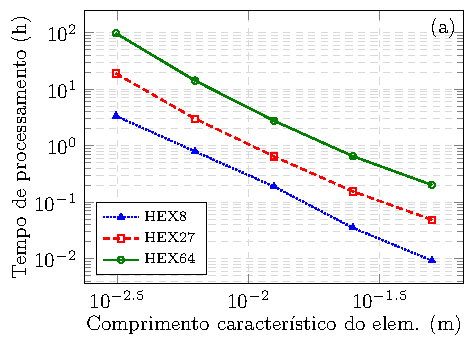
\includegraphics[scale=1.0]{Figuras/PTFE-cylinder-mesh/VepCylinder-Creep-Time-Conv.pdf}}\;\;{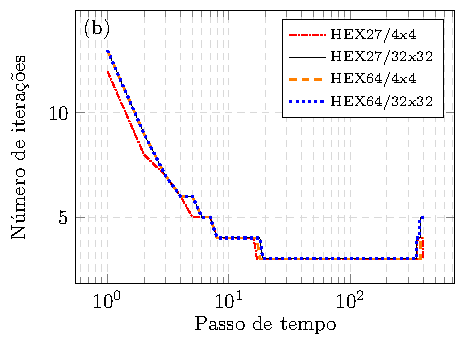
\includegraphics[scale=1.0]{Figuras/PTFE-cylinder-mesh/VepCylinder-Creep-iter.pdf}}
	%\caption*{\textbf{Fonte:} Elaborado pelo autor}
\end{figure}

\subsubsection{Ensaio de fluência com análise de convergência de tempo}

Novamente, considera-se um valor fixo de $21$ MPa para $p$, e um tempo de análise máximo de $10^6$ s. Entretanto, neste caso é feita uma análise de convergência para a discretização temporal. Toma-se uma malha fixa (HEX64/8x8), e $6$ diferentes discretizações temporais, com $100$, $200$, $400$, $800$, $1600$ e $3200$ passos de tempo. Novamente, os valores de $\Delta t$ em cada caso evoluem conforme uma progressão geométrica, com $\Delta t$ inicial inversamente proporcional ao número de passos. A razão da progressão geométrica, no entanto, não pode ser associada linearmente ao número de passos, e precisa ser calculada individualmente para cada discretização, utilizando o fato de que a soma dos termos da progressão deve ser igual ao tempo total de análise. Os dados completos das discretizações são mostrados na \autoref{tab:convergence-dt} para cada caso, bem como o deslocamento vertical mínimo (ocorrido no ponto A), o número total de iterações e o tempo de processamento. Nota-se que os resultados para $100$ passos de tempo não são incluídos, pois a discretização nesse caso não foi suficiente para prosseguir a análise, apresentando problemas de convergência já no primeiro passo.

\begin{table}[!h]
	\centering
	\scriptsize
	\caption{Análise de convergência para a discretização temporal do cilindro parcialmente comprimido sob fluência}
	\label{tab:convergence-dt}
	{\renewcommand{\arraystretch}{1.2}
		\begin{tabular}{cccccccc}
			\hline
			NPT & $\Delta t$ inicial (s) & razão da PG & $\Delta t$ final (s) & DESLY (cm) & IT-M & TP (s) & TP-EF (s) \\ \hline
			$100 $ & $5.13423970\cdot 10^{0}$ & $ 1.10427504$ & $9.44331542\cdot 10^{4}$ & --- & --- & --- & --- \\
			$200 $ & $2.56711985\cdot 10^{0}$ & $ 1.05069781$ & $4.82540019\cdot 10^{4}$ & $-2.64364$ & $4.6300$ & $   7274.8$ & $ 7062.8$ \\
			$400 $ & $1.28355992\cdot 10^{0}$ & $ 1.02500000$ & $2.43914962\cdot 10^{4}$ & $-2.63698$ & $3.2075$ & $   9932.6$ & $ 9719.4$ \\
			$800 $ & $6.41779962\cdot 10^{-1}$ & $ 1.01241411$ & $1.22625256\cdot 10^{4}$ & $-2.63267$ & $2.6938$ & $  16412.2$ & $16197.8$ \\
			$1600$ & $3.20889981\cdot 10^{-1}$ & $ 1.00618575$ & $6.14803972\cdot 10^{3}$ & $-2.62985$ & $2.5181$ & $  30134.4$ & $29917.5$ \\
			$3200$ & $1.60444991\cdot 10^{-1}$ & $ 1.00308757$ & $3.07822430\cdot 10^{3}$ & $-2.62786$ & $2.0241$ & $  48005.6$ & $47784.8$ \\ \hline
			\multicolumn{4}{l}{NPT = Número de passos de tempo} &  \multicolumn{4}{l}{DESLY = Deslocamento vertical mínimo}\\
			\multicolumn{4}{l}{IT-M = Número médio de iterações por passo de tempo} &  \multicolumn{4}{l}{TP = Tempo de processamento total}\\
			\multicolumn{7}{l}{TP-EF = Tempo de processamento descontando o pós e pré-processamento} \\
			\hline 
		\end{tabular}
	}
	%\caption*{\textbf{Fonte:} Elaborado pelo autor}
\end{table}

Como esperado, os tempos de processamento total e efetivos são maiores para os casos mais refinados, mas o número médio de iterações por passo de tempo é menor. Observa-se, no entanto, que os deslocamentos verticais mínimos não apresentam grandes divergências, apresentando um erro de apenas $0,6\%$ entre os casos com $200$ e $3200$ passos de tempo, o que é desprezível do ponto de vista prático. Esses resultados indicam que a discretização temporal aplicada possui pouca influência neste exemplo, desde que seja suficiente para garantir a convergência. Os erros com relação ao caso mais refinado ($3200$ passos) podem ser vistos na \cref{fig:cylinderCreep-time-conv}(a), e a evolução dos deslocamentos ao longo do tempo no ponto A é mostrada na \cref{fig:cylinderCreep-time-conv}(b) para alguns passos de tempo selecionados, sendo notável a similaridade entre os casos analisados.

\begin{figure}[!htb]
	\centering
	\caption{Análise de convergência para a discretização temporal do cilindro parcialmente comprimido sob fluência, incluindo (a) erro no deslocamento vertical do ponto A com relação à discretização temporal mais refinada, e (b) deslocamento vertical no ponto A ao longo do tempo}
	\label{fig:cylinderCreep-time-conv}
	{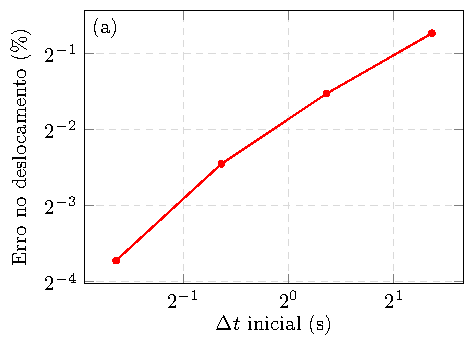
\includegraphics[scale=1.0]{Figuras/PTFE-cylinder-time/VepCylinderCreepTime-v-Conv.pdf}}\;{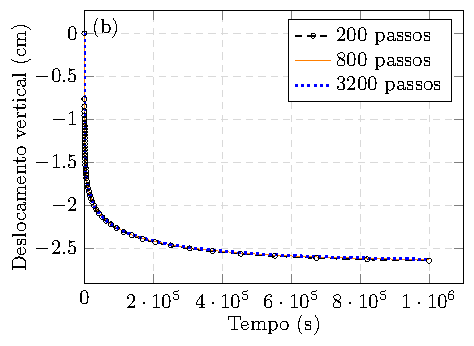
\includegraphics[scale=1.0]{Figuras/PTFE-cylinder-time/VepCylinderCreepTime-v.pdf}}
	%\caption*{\textbf{Fonte:} Elaborado pelo autor}
\end{figure}


\end{document}